\documentclass[twoside]{book}

% Packages required by doxygen
\usepackage{fixltx2e}
\usepackage{calc}
\usepackage{doxygen}
\usepackage{graphicx}
\usepackage[utf8]{inputenc}
\usepackage{makeidx}
\usepackage{multicol}
\usepackage{multirow}
\PassOptionsToPackage{warn}{textcomp}
\usepackage{textcomp}
\usepackage[nointegrals]{wasysym}
\usepackage[table]{xcolor}

% Font selection
\usepackage[T1]{fontenc}
\usepackage{mathptmx}
\usepackage[scaled=.90]{helvet}
\usepackage{courier}
\usepackage{amssymb}
\usepackage{sectsty}
\renewcommand{\familydefault}{\sfdefault}
\allsectionsfont{%
  \fontseries{bc}\selectfont%
  \color{darkgray}%
}
\renewcommand{\DoxyLabelFont}{%
  \fontseries{bc}\selectfont%
  \color{darkgray}%
}
\newcommand{\+}{\discretionary{\mbox{\scriptsize$\hookleftarrow$}}{}{}}

% Page & text layout
\usepackage{geometry}
\geometry{%
  a4paper,%
  top=2.5cm,%
  bottom=2.5cm,%
  left=2.5cm,%
  right=2.5cm%
}
\tolerance=750
\hfuzz=15pt
\hbadness=750
\setlength{\emergencystretch}{15pt}
\setlength{\parindent}{0cm}
\setlength{\parskip}{0.2cm}
\makeatletter
\renewcommand{\paragraph}{%
  \@startsection{paragraph}{4}{0ex}{-1.0ex}{1.0ex}{%
    \normalfont\normalsize\bfseries\SS@parafont%
  }%
}
\renewcommand{\subparagraph}{%
  \@startsection{subparagraph}{5}{0ex}{-1.0ex}{1.0ex}{%
    \normalfont\normalsize\bfseries\SS@subparafont%
  }%
}
\makeatother

% Headers & footers
\usepackage{fancyhdr}
\pagestyle{fancyplain}
\fancyhead[LE]{\fancyplain{}{\bfseries\thepage}}
\fancyhead[CE]{\fancyplain{}{}}
\fancyhead[RE]{\fancyplain{}{\bfseries\leftmark}}
\fancyhead[LO]{\fancyplain{}{\bfseries\rightmark}}
\fancyhead[CO]{\fancyplain{}{}}
\fancyhead[RO]{\fancyplain{}{\bfseries\thepage}}
\fancyfoot[LE]{\fancyplain{}{}}
\fancyfoot[CE]{\fancyplain{}{}}
\fancyfoot[RE]{\fancyplain{}{\bfseries\scriptsize Generated on Sun Dec 28 2014 15\+:51\+:54 for Machine Learning Final Project by Doxygen }}
\fancyfoot[LO]{\fancyplain{}{\bfseries\scriptsize Generated on Sun Dec 28 2014 15\+:51\+:54 for Machine Learning Final Project by Doxygen }}
\fancyfoot[CO]{\fancyplain{}{}}
\fancyfoot[RO]{\fancyplain{}{}}
\renewcommand{\footrulewidth}{0.4pt}
\renewcommand{\chaptermark}[1]{%
  \markboth{#1}{}%
}
\renewcommand{\sectionmark}[1]{%
  \markright{\thesection\ #1}%
}

% Indices & bibliography
\usepackage{natbib}
\usepackage[titles]{tocloft}
\setcounter{tocdepth}{3}
\setcounter{secnumdepth}{5}
\makeindex

% Hyperlinks (required, but should be loaded last)
\usepackage{ifpdf}
\ifpdf
  \usepackage[pdftex,pagebackref=true]{hyperref}
\else
  \usepackage[ps2pdf,pagebackref=true]{hyperref}
\fi
\hypersetup{%
  colorlinks=true,%
  linkcolor=blue,%
  citecolor=blue,%
  unicode%
}

% Custom commands
\newcommand{\clearemptydoublepage}{%
  \newpage{\pagestyle{empty}\cleardoublepage}%
}


%===== C O N T E N T S =====

\begin{document}

% Titlepage & ToC
\hypersetup{pageanchor=false,
             bookmarks=true,
             bookmarksnumbered=true,
             pdfencoding=unicode
            }
\pagenumbering{roman}
\begin{titlepage}
\vspace*{7cm}
\begin{center}%
{\Large Machine Learning Final Project }\\
\vspace*{1cm}
{\large Generated by Doxygen 1.8.8}\\
\vspace*{0.5cm}
{\small Sun Dec 28 2014 15:51:54}\\
\end{center}
\end{titlepage}
\clearemptydoublepage
\tableofcontents
\clearemptydoublepage
\pagenumbering{arabic}
\hypersetup{pageanchor=true}

%--- Begin generated contents ---
\chapter{Main Page}
\label{index}\hypertarget{index}{}The {\bfseries goal} is to design a {\itshape labeled two class data set} of 10-\/dimensional vectors that has test set classification accuracy less than 60\% on some popular classifiers. However, our decision rule was designed such that it can perform with greater than 90\% accuracy on the test set.


\begin{DoxyItemize}
\item {\bfseries Authors}\+: Carlos Jaramillo {\bfseries and} Juan Pablo Munoz
\item {\bfseries Contact}\+: \href{mailto:cjaramillo@gc.cuny.edu}{\tt cjaramillo@gc.\+cuny.\+edu} {\bfseries and} \href{mailto:jpablomch@gmail.com}{\tt jpablomch@gmail.\+com}
\end{DoxyItemize}

{\itshape Copyright (C)} 2014 under the {\itshape Gnu Public License version 2 (G\+P\+L2)}

\subsection*{Overview}

\subsubsection*{Data Set Generation}

{\ttfamily \hyperlink{data__generation_8py}{data\+\_\+generation.\+py}} is a {\itshape toolbox} written in Python for data set generation satisfying the problem specifications. We generate a data set of 100,000 10-\/dimensional vectors (components), where 3 out them are relevant.

Decision rules and data set generation using 10 components and discrete values (from 0 to 9) for supervised learning \hyperlink{namespacelearning__driver}{learning\+\_\+driver}. The number of decision rules is reduced exponentially based upon the level of \hyperlink{namespacemate__learning}{mate\+\_\+learning} (grouping of values) applied across the selected relevant components.

\subsubsection*{Learning Method}

Supervised Learning method for binary classification based on mating (grouping of values) across the supplied data set of components and classification labels. The learning algorithm is implemented in '\hyperlink{mate__learning_8py}{mate\+\_\+learning.\+py}`. It consists of exhausting all the possibilities as long as accuracy of correct classification can be increased.

We define a {\ttfamily Mate\+Finder} class for the particular binary classification problem based on mates (usually groups of 2 -\/ pairs) across each component of a discrete-\/valued data set. The {\ttfamily Mate\+Finder} class provides procedures such as the removal of irrelevant components (selection of relevant components), as well as essential learning (training and validation) and testing procedures from learned decision tables of pairs.

Once a {\ttfamily Mate\+Finder} object has been instantiated through the constructor, the interfacing methods employed by an external classifier are\+: {\ttfamily learn\+\_\+by\+\_\+mate\+\_\+discovery()} and {\ttfamily compute\+\_\+prediction\+\_\+accuracy()}

The program driving the learning from data and estimating the accuracy of the learned decision rule on the testing set is driven by {\ttfamily \hyperlink{learning__driver_8py}{learning\+\_\+driver.\+py}}

\subsection*{Installing}

\subsubsection*{From source}

It's {\bfseries Python}! Only the \href{http://numpy.org}{\tt Numpy} module is required.

After fulfilling the module dependencies, just run the scripts, such as\+: \begin{DoxyVerb}$ python data_generation.py
\end{DoxyVerb}


\subsection*{Wish List}


\begin{DoxyItemize}
\item Gimme some!
\end{DoxyItemize}

\subsection*{More info}

$\ast$$\ast$$\ast$\+Documentation$\ast$$\ast$$\ast$\+: can be found in the 'docs' folder or regenerated via \href{http://code.foosel.org/doxypy}{\tt doxypy} 
\chapter{Namespace Index}
\section{Namespace List}
Here is a list of all namespaces with brief descriptions\+:\begin{DoxyCompactList}
\item\contentsline{section}{\hyperlink{namespacecommon__tools}{common\+\_\+tools} }{\pageref{namespacecommon__tools}}{}
\item\contentsline{section}{\hyperlink{namespacedata__generation}{data\+\_\+generation} }{\pageref{namespacedata__generation}}{}
\item\contentsline{section}{\hyperlink{namespacelearning__driver}{learning\+\_\+driver} }{\pageref{namespacelearning__driver}}{}
\item\contentsline{section}{\hyperlink{namespacemate__learning}{mate\+\_\+learning} }{\pageref{namespacemate__learning}}{}
\end{DoxyCompactList}

\chapter{Hierarchical Index}
\section{Class Hierarchy}
This inheritance list is sorted roughly, but not completely, alphabetically\+:\begin{DoxyCompactList}
\item object\begin{DoxyCompactList}
\item \contentsline{section}{mate\+\_\+learning.\+Mate\+Finder}{\pageref{classmate__learning_1_1_mate_finder}}{}
\end{DoxyCompactList}
\end{DoxyCompactList}

\chapter{Class Index}
\section{Class List}
Here are the classes, structs, unions and interfaces with brief descriptions\+:\begin{DoxyCompactList}
\item\contentsline{section}{\hyperlink{classmate__learning_1_1_mate_finder}{mate\+\_\+learning.\+Mate\+Finder} \\*Used for the particular binary classification problem based on mates (usually groups of 2 -\/ pairs) across each component of a discrete-\/valued data set }{\pageref{classmate__learning_1_1_mate_finder}}{}
\end{DoxyCompactList}

\chapter{File Index}
\section{File List}
Here is a list of all files with brief descriptions\+:\begin{DoxyCompactList}
\item\contentsline{section}{\hyperlink{common__tools_8py}{common\+\_\+tools.\+py} }{\pageref{common__tools_8py}}{}
\item\contentsline{section}{\hyperlink{data__generation_8py}{data\+\_\+generation.\+py} }{\pageref{data__generation_8py}}{}
\item\contentsline{section}{\hyperlink{learning__driver_8py}{learning\+\_\+driver.\+py} }{\pageref{learning__driver_8py}}{}
\item\contentsline{section}{\hyperlink{mate__learning_8py}{mate\+\_\+learning.\+py} }{\pageref{mate__learning_8py}}{}
\end{DoxyCompactList}

\chapter{Namespace Documentation}
\hypertarget{namespacecommon__tools}{\section{common\+\_\+tools Namespace Reference}
\label{namespacecommon__tools}\index{common\+\_\+tools@{common\+\_\+tools}}
}
\subsection*{Functions}
\begin{DoxyCompactItemize}
\item 
def \hyperlink{namespacecommon__tools_a99127ed524481a987098d0b646248ac7}{get\+\_\+namestr}
\begin{DoxyCompactList}\small\item\em Finds and returns the variable name for the object instance in question in the desired namespace. \end{DoxyCompactList}\item 
def \hyperlink{namespacecommon__tools_a31bbee936ad9ee3f26d71ba58c435125}{save\+\_\+obj\+\_\+in\+\_\+pickle}
\item 
def \hyperlink{namespacecommon__tools_ae02aaf0ee60b16dd5d22f2e3f20fd9e6}{load\+\_\+obj\+\_\+from\+\_\+pickle}
\item 
def \hyperlink{namespacecommon__tools_ae5d41b7419e727e4389ae0a37f684a7f}{save\+\_\+dataset\+\_\+to\+\_\+pickle}
\item 
def \hyperlink{namespacecommon__tools_a38d5594d132460ab544508a860c74840}{load\+\_\+dataset\+\_\+from\+\_\+pickle}
\item 
def \hyperlink{namespacecommon__tools_a7987ebb2fe78986ee5bd276b9ca23b54}{read\+\_\+data}
\item 
def \hyperlink{namespacecommon__tools_aaa8d6759ce602c7555a4f247523a7b17}{filter\+\_\+irrelevant\+\_\+features}
\item 
def \hyperlink{namespacecommon__tools_a0f555f84922eeeeef319b1c696a53398}{pdf}
\item 
def \hyperlink{namespacecommon__tools_affa5e6fbad6fb93eafef8208833518ac}{reverse\+\_\+axis\+\_\+elems}
\item 
def \hyperlink{namespacecommon__tools_a3c8bdaaa99b2ded40cae5110fe429dc9}{rms}
\item 
def \hyperlink{namespacecommon__tools_ac61789513b883ed1c0519fafbc04db09}{nanrms}
\begin{DoxyCompactList}\small\item\em If you have nans in your data, you can do. \end{DoxyCompactList}\item 
def \hyperlink{namespacecommon__tools_af05b64800eee31edb0e18ff46d0163f5}{weighted\+\_\+avg\+\_\+and\+\_\+std}
\begin{DoxyCompactList}\small\item\em Return the weighted average and standard deviation. \end{DoxyCompactList}\item 
def \hyperlink{namespacecommon__tools_a6176dbbdc3e730a07138b14a5cd8f48e}{mean\+\_\+and\+\_\+std}
\begin{DoxyCompactList}\small\item\em Return the arithmetic mean or unweighted average and the standard deviation. \end{DoxyCompactList}\end{DoxyCompactItemize}


\subsection{Function Documentation}
\hypertarget{namespacecommon__tools_aaa8d6759ce602c7555a4f247523a7b17}{\index{common\+\_\+tools@{common\+\_\+tools}!filter\+\_\+irrelevant\+\_\+features@{filter\+\_\+irrelevant\+\_\+features}}
\index{filter\+\_\+irrelevant\+\_\+features@{filter\+\_\+irrelevant\+\_\+features}!common\+\_\+tools@{common\+\_\+tools}}
\subsubsection[{filter\+\_\+irrelevant\+\_\+features}]{\setlength{\rightskip}{0pt plus 5cm}def common\+\_\+tools.\+filter\+\_\+irrelevant\+\_\+features (
\begin{DoxyParamCaption}
\item[{}]{feature\+\_\+data, }
\item[{}]{labels, }
\item[{}]{wanted\+\_\+num\+\_\+of\+\_\+features, }
\item[{}]{use\+\_\+chi2 = {\ttfamily True}}
\end{DoxyParamCaption}
)}}\label{namespacecommon__tools_aaa8d6759ce602c7555a4f247523a7b17}

\begin{DoxyParams}{Parameters}
{\em use\+\_\+sklearn} & Indicates whether the filtering is done with scikit-\/learn's Select\+K\+Besr or a custom bruteforce procedure. \\
\hline
\end{DoxyParams}


Definition at line 110 of file common\+\_\+tools.\+py.

\hypertarget{namespacecommon__tools_a99127ed524481a987098d0b646248ac7}{\index{common\+\_\+tools@{common\+\_\+tools}!get\+\_\+namestr@{get\+\_\+namestr}}
\index{get\+\_\+namestr@{get\+\_\+namestr}!common\+\_\+tools@{common\+\_\+tools}}
\subsubsection[{get\+\_\+namestr}]{\setlength{\rightskip}{0pt plus 5cm}def common\+\_\+tools.\+get\+\_\+namestr (
\begin{DoxyParamCaption}
\item[{}]{obj, }
\item[{}]{namespace}
\end{DoxyParamCaption}
)}}\label{namespacecommon__tools_a99127ed524481a987098d0b646248ac7}


Finds and returns the variable name for the object instance in question in the desired namespace. 

For example \begin{DoxyVerb}>>> get_namestr(my_wow, globals())
Out: 'my_wow'\end{DoxyVerb}
 

Definition at line 23 of file common\+\_\+tools.\+py.



Referenced by load\+\_\+obj\+\_\+from\+\_\+pickle(), and save\+\_\+obj\+\_\+in\+\_\+pickle().

\hypertarget{namespacecommon__tools_a38d5594d132460ab544508a860c74840}{\index{common\+\_\+tools@{common\+\_\+tools}!load\+\_\+dataset\+\_\+from\+\_\+pickle@{load\+\_\+dataset\+\_\+from\+\_\+pickle}}
\index{load\+\_\+dataset\+\_\+from\+\_\+pickle@{load\+\_\+dataset\+\_\+from\+\_\+pickle}!common\+\_\+tools@{common\+\_\+tools}}
\subsubsection[{load\+\_\+dataset\+\_\+from\+\_\+pickle}]{\setlength{\rightskip}{0pt plus 5cm}def common\+\_\+tools.\+load\+\_\+dataset\+\_\+from\+\_\+pickle (
\begin{DoxyParamCaption}
\item[{}]{filename\+\_\+prefix}
\end{DoxyParamCaption}
)}}\label{namespacecommon__tools_a38d5594d132460ab544508a860c74840}


Definition at line 51 of file common\+\_\+tools.\+py.



References load\+\_\+obj\+\_\+from\+\_\+pickle().



Referenced by learning\+\_\+driver.\+classify\+\_\+dataset().

\hypertarget{namespacecommon__tools_ae02aaf0ee60b16dd5d22f2e3f20fd9e6}{\index{common\+\_\+tools@{common\+\_\+tools}!load\+\_\+obj\+\_\+from\+\_\+pickle@{load\+\_\+obj\+\_\+from\+\_\+pickle}}
\index{load\+\_\+obj\+\_\+from\+\_\+pickle@{load\+\_\+obj\+\_\+from\+\_\+pickle}!common\+\_\+tools@{common\+\_\+tools}}
\subsubsection[{load\+\_\+obj\+\_\+from\+\_\+pickle}]{\setlength{\rightskip}{0pt plus 5cm}def common\+\_\+tools.\+load\+\_\+obj\+\_\+from\+\_\+pickle (
\begin{DoxyParamCaption}
\item[{}]{filename, }
\item[{}]{namespace = {\ttfamily None}}
\end{DoxyParamCaption}
)}}\label{namespacecommon__tools_ae02aaf0ee60b16dd5d22f2e3f20fd9e6}


Definition at line 40 of file common\+\_\+tools.\+py.



References get\+\_\+namestr().



Referenced by load\+\_\+dataset\+\_\+from\+\_\+pickle().

\hypertarget{namespacecommon__tools_a6176dbbdc3e730a07138b14a5cd8f48e}{\index{common\+\_\+tools@{common\+\_\+tools}!mean\+\_\+and\+\_\+std@{mean\+\_\+and\+\_\+std}}
\index{mean\+\_\+and\+\_\+std@{mean\+\_\+and\+\_\+std}!common\+\_\+tools@{common\+\_\+tools}}
\subsubsection[{mean\+\_\+and\+\_\+std}]{\setlength{\rightskip}{0pt plus 5cm}def common\+\_\+tools.\+mean\+\_\+and\+\_\+std (
\begin{DoxyParamCaption}
\item[{}]{values}
\end{DoxyParamCaption}
)}}\label{namespacecommon__tools_a6176dbbdc3e730a07138b14a5cd8f48e}


Return the arithmetic mean or unweighted average and the standard deviation. 


\begin{DoxyParams}{Parameters}
{\em values} & Numpy ndarrays of values \\
\hline
\end{DoxyParams}


Definition at line 170 of file common\+\_\+tools.\+py.

\hypertarget{namespacecommon__tools_ac61789513b883ed1c0519fafbc04db09}{\index{common\+\_\+tools@{common\+\_\+tools}!nanrms@{nanrms}}
\index{nanrms@{nanrms}!common\+\_\+tools@{common\+\_\+tools}}
\subsubsection[{nanrms}]{\setlength{\rightskip}{0pt plus 5cm}def common\+\_\+tools.\+nanrms (
\begin{DoxyParamCaption}
\item[{}]{x, }
\item[{}]{axis = {\ttfamily None}}
\end{DoxyParamCaption}
)}}\label{namespacecommon__tools_ac61789513b883ed1c0519fafbc04db09}


If you have nans in your data, you can do. 



Definition at line 150 of file common\+\_\+tools.\+py.

\hypertarget{namespacecommon__tools_a0f555f84922eeeeef319b1c696a53398}{\index{common\+\_\+tools@{common\+\_\+tools}!pdf@{pdf}}
\index{pdf@{pdf}!common\+\_\+tools@{common\+\_\+tools}}
\subsubsection[{pdf}]{\setlength{\rightskip}{0pt plus 5cm}def common\+\_\+tools.\+pdf (
\begin{DoxyParamCaption}
\item[{}]{point, }
\item[{}]{cons, }
\item[{}]{mean, }
\item[{}]{det\+\_\+sigma}
\end{DoxyParamCaption}
)}}\label{namespacecommon__tools_a0f555f84922eeeeef319b1c696a53398}


Definition at line 123 of file common\+\_\+tools.\+py.

\hypertarget{namespacecommon__tools_a7987ebb2fe78986ee5bd276b9ca23b54}{\index{common\+\_\+tools@{common\+\_\+tools}!read\+\_\+data@{read\+\_\+data}}
\index{read\+\_\+data@{read\+\_\+data}!common\+\_\+tools@{common\+\_\+tools}}
\subsubsection[{read\+\_\+data}]{\setlength{\rightskip}{0pt plus 5cm}def common\+\_\+tools.\+read\+\_\+data (
\begin{DoxyParamCaption}
\item[{}]{filename, }
\item[{}]{delimiter = {\ttfamily \char`\"{}}, }
\item[{}]{feature\+\_\+indices = {\ttfamily None}, }
\item[{}]{use\+\_\+string\+\_\+labels = {\ttfamily True}, }
\item[{}]{given\+\_\+string\+\_\+labels = {\ttfamily False}, }
\item[{}]{num\+\_\+components = {\ttfamily 10}, }
\item[{}]{dtype = {\ttfamily 'uint8'}, }
\item[{}]{has\+\_\+header = {\ttfamily True}, }
\item[{}]{shuffle\+\_\+rows = {\ttfamily False}}
\end{DoxyParamCaption}
)}}\label{namespacecommon__tools_a7987ebb2fe78986ee5bd276b9ca23b54}

\begin{DoxyParams}{Parameters}
{\em filename} & the database filename path \\
\hline
{\em delimiter} & the string usefile delimeter (e.\+g. \char`\"{},\char`\"{}) \\
\hline
{\em feature\+\_\+indices} & The index of the columns for the desired indices. If nothing is passed, then all features are used. \\
\hline
{\em use\+\_\+string\+\_\+labels} & indicates whether labels are kept as strings, or if False, they should be indexed instead \\
\hline
{\em given\+\_\+string\+\_\+labels} & indicates whether class labels are strings. Use False (default) to imply the use of digit labels \\
\hline
{\em num\+\_\+components} & number of columns (feature dimensions) in the file. \\
\hline
\end{DoxyParams}
\begin{DoxyReturn}{Returns}
the np array of features and the single-\/column array of the labels from the dataset being read. 
\end{DoxyReturn}


Definition at line 65 of file common\+\_\+tools.\+py.



Referenced by learning\+\_\+driver.\+classify\+\_\+dataset(), and learning\+\_\+driver.\+learn\+\_\+model\+\_\+naive\+\_\+bayes().

\hypertarget{namespacecommon__tools_affa5e6fbad6fb93eafef8208833518ac}{\index{common\+\_\+tools@{common\+\_\+tools}!reverse\+\_\+axis\+\_\+elems@{reverse\+\_\+axis\+\_\+elems}}
\index{reverse\+\_\+axis\+\_\+elems@{reverse\+\_\+axis\+\_\+elems}!common\+\_\+tools@{common\+\_\+tools}}
\subsubsection[{reverse\+\_\+axis\+\_\+elems}]{\setlength{\rightskip}{0pt plus 5cm}def common\+\_\+tools.\+reverse\+\_\+axis\+\_\+elems (
\begin{DoxyParamCaption}
\item[{}]{arr, }
\item[{}]{k = {\ttfamily 0}}
\end{DoxyParamCaption}
)}}\label{namespacecommon__tools_affa5e6fbad6fb93eafef8208833518ac}

\begin{DoxyParams}{Parameters}
{\em arr} & the numpy ndarray to be reversed \\
\hline
{\em k} & The axis to be reversed Reverse the order of rows\+: set axis k=0 Reverse the order of columns\+: set axis k=1\\
\hline
\end{DoxyParams}
\begin{DoxyReturn}{Returns}
\+: the reversed numpy array 
\end{DoxyReturn}


Definition at line 138 of file common\+\_\+tools.\+py.

\hypertarget{namespacecommon__tools_a3c8bdaaa99b2ded40cae5110fe429dc9}{\index{common\+\_\+tools@{common\+\_\+tools}!rms@{rms}}
\index{rms@{rms}!common\+\_\+tools@{common\+\_\+tools}}
\subsubsection[{rms}]{\setlength{\rightskip}{0pt plus 5cm}def common\+\_\+tools.\+rms (
\begin{DoxyParamCaption}
\item[{}]{x, }
\item[{}]{axis = {\ttfamily None}}
\end{DoxyParamCaption}
)}}\label{namespacecommon__tools_a3c8bdaaa99b2ded40cae5110fe429dc9}


Definition at line 142 of file common\+\_\+tools.\+py.

\hypertarget{namespacecommon__tools_ae5d41b7419e727e4389ae0a37f684a7f}{\index{common\+\_\+tools@{common\+\_\+tools}!save\+\_\+dataset\+\_\+to\+\_\+pickle@{save\+\_\+dataset\+\_\+to\+\_\+pickle}}
\index{save\+\_\+dataset\+\_\+to\+\_\+pickle@{save\+\_\+dataset\+\_\+to\+\_\+pickle}!common\+\_\+tools@{common\+\_\+tools}}
\subsubsection[{save\+\_\+dataset\+\_\+to\+\_\+pickle}]{\setlength{\rightskip}{0pt plus 5cm}def common\+\_\+tools.\+save\+\_\+dataset\+\_\+to\+\_\+pickle (
\begin{DoxyParamCaption}
\item[{}]{all\+\_\+features\+\_\+data, }
\item[{}]{all\+\_\+classes, }
\item[{}]{filename\+\_\+prefix}
\end{DoxyParamCaption}
)}}\label{namespacecommon__tools_ae5d41b7419e727e4389ae0a37f684a7f}


Definition at line 48 of file common\+\_\+tools.\+py.



References save\+\_\+obj\+\_\+in\+\_\+pickle().



Referenced by learning\+\_\+driver.\+classify\+\_\+dataset().

\hypertarget{namespacecommon__tools_a31bbee936ad9ee3f26d71ba58c435125}{\index{common\+\_\+tools@{common\+\_\+tools}!save\+\_\+obj\+\_\+in\+\_\+pickle@{save\+\_\+obj\+\_\+in\+\_\+pickle}}
\index{save\+\_\+obj\+\_\+in\+\_\+pickle@{save\+\_\+obj\+\_\+in\+\_\+pickle}!common\+\_\+tools@{common\+\_\+tools}}
\subsubsection[{save\+\_\+obj\+\_\+in\+\_\+pickle}]{\setlength{\rightskip}{0pt plus 5cm}def common\+\_\+tools.\+save\+\_\+obj\+\_\+in\+\_\+pickle (
\begin{DoxyParamCaption}
\item[{}]{obj\+\_\+instance, }
\item[{}]{filename, }
\item[{}]{namespace = {\ttfamily None}}
\end{DoxyParamCaption}
)}}\label{namespacecommon__tools_a31bbee936ad9ee3f26d71ba58c435125}


Definition at line 33 of file common\+\_\+tools.\+py.



References get\+\_\+namestr().



Referenced by save\+\_\+dataset\+\_\+to\+\_\+pickle().

\hypertarget{namespacecommon__tools_af05b64800eee31edb0e18ff46d0163f5}{\index{common\+\_\+tools@{common\+\_\+tools}!weighted\+\_\+avg\+\_\+and\+\_\+std@{weighted\+\_\+avg\+\_\+and\+\_\+std}}
\index{weighted\+\_\+avg\+\_\+and\+\_\+std@{weighted\+\_\+avg\+\_\+and\+\_\+std}!common\+\_\+tools@{common\+\_\+tools}}
\subsubsection[{weighted\+\_\+avg\+\_\+and\+\_\+std}]{\setlength{\rightskip}{0pt plus 5cm}def common\+\_\+tools.\+weighted\+\_\+avg\+\_\+and\+\_\+std (
\begin{DoxyParamCaption}
\item[{}]{values, }
\item[{}]{weights}
\end{DoxyParamCaption}
)}}\label{namespacecommon__tools_af05b64800eee31edb0e18ff46d0163f5}


Return the weighted average and standard deviation. 

values, weights -- Numpy ndarrays with the same shape. 

Definition at line 159 of file common\+\_\+tools.\+py.


\hypertarget{namespacedata__generation}{\section{data\+\_\+generation Namespace Reference}
\label{namespacedata__generation}\index{data\+\_\+generation@{data\+\_\+generation}}
}
\subsection*{Functions}
\begin{DoxyCompactItemize}
\item 
def \hyperlink{namespacedata__generation_a723f3547cdfa6066526de7b8964a0a49}{generate\+\_\+rules}
\begin{DoxyCompactList}\small\item\em Generate \hyperlink{namespacelearning__driver}{learning\+\_\+driver} rules as a big L\+U\+T where irrelevant values get an invalid value of -\/1 Valid values for components are only nonnegative integers in the interval \mbox{[}0, 9\mbox{]}. \end{DoxyCompactList}\item 
def \hyperlink{namespacedata__generation_a0a700e2749ed935a31ac58217132cb76}{generate\+\_\+dataset}
\begin{DoxyCompactList}\small\item\em Irrelevant components are filled up with random values from a uniform distribution Last, the generated instance vectors (measurement records or rows including their associated class label) of the data set are shuffled and returned as the final result. \end{DoxyCompactList}\end{DoxyCompactItemize}
\subsection*{Variables}
\begin{DoxyCompactItemize}
\item 
list \hyperlink{namespacedata__generation_ab52d553b1eb5f4c6d065e0435753addc}{class\+\_\+labels} = \mbox{[}0, 1\mbox{]}
\item 
list \hyperlink{namespacedata__generation_a1c4e107080b11e6ef67edd30bfb93b05}{instances\+\_\+percentages} = \mbox{[}50, 50\mbox{]}
\item 
list \hyperlink{namespacedata__generation_afa9b1b91a7860372739bca028f41263b}{relevant\+\_\+components} = \mbox{[}0, 1, 8\mbox{]}
\item 
int \hyperlink{namespacedata__generation_a963ce4f506a2b3bb6acb94915445f716}{total\+\_\+num\+\_\+of\+\_\+instances} = 100000
\item 
int \hyperlink{namespacedata__generation_ad68308d6e9bf4bd2485a44ce0c52315c}{num\+\_\+of\+\_\+components} = 10
\item 
list \hyperlink{namespacedata__generation_a345ef2cc135025dccbfbba8502ba6d8d}{dataset\+\_\+header} = \mbox{[}\char`\"{}d\char`\"{} + str(fname + 1) for fname in range(\hyperlink{namespacedata__generation_ad68308d6e9bf4bd2485a44ce0c52315c}{num\+\_\+of\+\_\+components})\mbox{]}
\item 
string \hyperlink{namespacedata__generation_ad7ee72f39a9a602967e77e4da382566a}{path\+\_\+to\+\_\+output\+\_\+files} = \char`\"{}./Input\+Data/\char`\"{}
\item 
\hyperlink{namespacedata__generation_abf6964c9992abb3c8c479fa568833f1c}{will\+\_\+generate\+\_\+rules} = True
\item 
int \hyperlink{namespacedata__generation_adf1cda3bf67a0646998d7ad03f8d1337}{quant\+\_\+levels} = 5
\item 
\hyperlink{namespacedata__generation_ae8c6a78af0481f316865220c829b86d2}{save\+\_\+class\+\_\+as\+\_\+string} = True
\item 
tuple \hyperlink{namespacedata__generation_a0750f715835d704f388842c370b48499}{k\+\_\+comp\+\_\+str} = str(len(\hyperlink{namespacedata__generation_afa9b1b91a7860372739bca028f41263b}{relevant\+\_\+components}))
\item 
string \hyperlink{namespacedata__generation_ad5e85da3fcf335e51b7dacc9404e221b}{filename\+\_\+time} = \hyperlink{namespacedata__generation_a0750f715835d704f388842c370b48499}{k\+\_\+comp\+\_\+str}+\char`\"{}rel\+\_\+components-\/quantized\+\_\+butterfly-\/2014-\/12-\/27\char`\"{}
\item 
list \hyperlink{namespacedata__generation_a4f985887946a96aa23f5ee6af6ec33fd}{custom\+\_\+fmt} = \mbox{[}\char`\"{}\%s\char`\"{} for fname in range(\hyperlink{namespacedata__generation_ad68308d6e9bf4bd2485a44ce0c52315c}{num\+\_\+of\+\_\+components})\mbox{]}
\item 
tuple \hyperlink{namespacedata__generation_a18484efee600914bdb61f4082236d2ba}{rules} = \hyperlink{namespacedata__generation_a723f3547cdfa6066526de7b8964a0a49}{generate\+\_\+rules}(\hyperlink{namespacedata__generation_ab52d553b1eb5f4c6d065e0435753addc}{class\+\_\+labels}, \hyperlink{namespacedata__generation_ad68308d6e9bf4bd2485a44ce0c52315c}{num\+\_\+of\+\_\+components}, \hyperlink{namespacedata__generation_afa9b1b91a7860372739bca028f41263b}{relevant\+\_\+components}, \hyperlink{namespacedata__generation_adf1cda3bf67a0646998d7ad03f8d1337}{quant\+\_\+levels})
\item 
tuple \hyperlink{namespacedata__generation_a4f08e445af07b6a8af849d8fd67dfbc9}{now} = datetime.\+datetime.\+now()
\item 
string \hyperlink{namespacedata__generation_a2fd941c060f70244057a35a916a6a9d7}{rules\+\_\+filename} = \hyperlink{namespacedata__generation_ad7ee72f39a9a602967e77e4da382566a}{path\+\_\+to\+\_\+output\+\_\+files}+\char`\"{}rules-\/\char`\"{}
\item 
tuple \hyperlink{namespacedata__generation_aa245bd201fe9810d8a8d8d615c4915ee}{rules\+\_\+labels} = np.\+where(\hyperlink{namespacedata__generation_a18484efee600914bdb61f4082236d2ba}{rules}\mbox{[}\+:, -\/1\mbox{]} == 0, 'A', 'B')
\item 
tuple \hyperlink{namespacedata__generation_a1e7ee3bfd1df183fdb922bbc4e93d12e}{rules\+\_\+as\+\_\+str} = np.\+hstack((\hyperlink{namespacedata__generation_a18484efee600914bdb61f4082236d2ba}{rules}\mbox{[}\+:, \+:-\/1\mbox{]}.astype('S2'), rules\+\_\+labels.\+reshape(-\/1, 1)))
\item 
\hyperlink{namespacedata__generation_a65cdb95b35877149855b39ef209ada8e}{use\+\_\+string\+\_\+labels} = \hyperlink{namespacedata__generation_ae8c6a78af0481f316865220c829b86d2}{save\+\_\+class\+\_\+as\+\_\+string},\textbackslash{}
\item 
string \hyperlink{namespacedata__generation_a577eb8996c6d5ddad4042ac0552f5aaa}{num\+\_\+components} = 'int8'
\item 
tuple \hyperlink{namespacedata__generation_ad3ed025b5adf596264de6710e2b25996}{dataset} = \hyperlink{namespacedata__generation_a0a700e2749ed935a31ac58217132cb76}{generate\+\_\+dataset}(\hyperlink{namespacedata__generation_a18484efee600914bdb61f4082236d2ba}{rules}, \hyperlink{namespacedata__generation_afa9b1b91a7860372739bca028f41263b}{relevant\+\_\+components}, \hyperlink{namespacedata__generation_a963ce4f506a2b3bb6acb94915445f716}{total\+\_\+num\+\_\+of\+\_\+instances}, \hyperlink{namespacedata__generation_a1c4e107080b11e6ef67edd30bfb93b05}{instances\+\_\+percentages}, \hyperlink{namespacedata__generation_adf1cda3bf67a0646998d7ad03f8d1337}{quant\+\_\+levels})
\item 
string \hyperlink{namespacedata__generation_a65485117b9e70dfb1f8046f6bf221338}{dataset\+\_\+filename} = \hyperlink{namespacedata__generation_ad7ee72f39a9a602967e77e4da382566a}{path\+\_\+to\+\_\+output\+\_\+files}+\char`\"{}dataset-\/\char`\"{}
\item 
tuple \hyperlink{namespacedata__generation_ad88beaf5c221ab8fbfeac2fd7aaafe65}{dataset\+\_\+labels} = np.\+where(\hyperlink{namespacedata__generation_ad3ed025b5adf596264de6710e2b25996}{dataset}\mbox{[}\+:, -\/1\mbox{]} == 0, 'A', 'B')
\item 
tuple \hyperlink{namespacedata__generation_ad40c466460ec72a381167165d38a2c07}{dataset\+\_\+as\+\_\+str} = np.\+hstack((\hyperlink{namespacedata__generation_ad3ed025b5adf596264de6710e2b25996}{dataset}\mbox{[}\+:, \+:-\/1\mbox{]}.astype('S2'), dataset\+\_\+labels.\+reshape(-\/1, 1)))
\end{DoxyCompactItemize}


\subsection{Function Documentation}
\hypertarget{namespacedata__generation_a0a700e2749ed935a31ac58217132cb76}{\index{data\+\_\+generation@{data\+\_\+generation}!generate\+\_\+dataset@{generate\+\_\+dataset}}
\index{generate\+\_\+dataset@{generate\+\_\+dataset}!data\+\_\+generation@{data\+\_\+generation}}
\subsubsection[{generate\+\_\+dataset}]{\setlength{\rightskip}{0pt plus 5cm}def data\+\_\+generation.\+generate\+\_\+dataset (
\begin{DoxyParamCaption}
\item[{}]{rules, }
\item[{}]{relevant\+\_\+components, }
\item[{}]{total\+\_\+num\+\_\+of\+\_\+instances, }
\item[{}]{instances\+\_\+percentages, }
\item[{}]{num\+\_\+of\+\_\+groups}
\end{DoxyParamCaption}
)}}\label{namespacedata__generation_a0a700e2749ed935a31ac58217132cb76}


Irrelevant components are filled up with random values from a uniform distribution Last, the generated instance vectors (measurement records or rows including their associated class label) of the data set are shuffled and returned as the final result. 


\begin{DoxyParams}{Parameters}
{\em rules} & Numpy ndarray of rules organized as a 2\+D table of components and classes (last column) \\
\hline
{\em relevant\+\_\+components} & The list of relevant components \\
\hline
{\em total\+\_\+num\+\_\+of\+\_\+instances} & The desired number of instances \\
\hline
{\em instances\+\_\+percentages} & The split (percentage-\/wise) of instances from each category (class) \\
\hline
{\em num\+\_\+of\+\_\+groups} & If set to 10, then grouping doesn't have an effect because groups would have a single element each.\\
\hline
\end{DoxyParams}
\begin{DoxyReturn}{Returns}
\+: The generated data set as a numpy array in which the last column corresponds to \hyperlink{namespacelearning__driver}{learning\+\_\+driver} labels. 
\end{DoxyReturn}


Definition at line 80 of file data\+\_\+generation.\+py.

\hypertarget{namespacedata__generation_a723f3547cdfa6066526de7b8964a0a49}{\index{data\+\_\+generation@{data\+\_\+generation}!generate\+\_\+rules@{generate\+\_\+rules}}
\index{generate\+\_\+rules@{generate\+\_\+rules}!data\+\_\+generation@{data\+\_\+generation}}
\subsubsection[{generate\+\_\+rules}]{\setlength{\rightskip}{0pt plus 5cm}def data\+\_\+generation.\+generate\+\_\+rules (
\begin{DoxyParamCaption}
\item[{}]{class\+\_\+labels, }
\item[{}]{num\+\_\+of\+\_\+components, }
\item[{}]{relevant\+\_\+components, }
\item[{}]{num\+\_\+of\+\_\+groups}
\end{DoxyParamCaption}
)}}\label{namespacedata__generation_a723f3547cdfa6066526de7b8964a0a49}


Generate \hyperlink{namespacelearning__driver}{learning\+\_\+driver} rules as a big L\+U\+T where irrelevant values get an invalid value of -\/1 Valid values for components are only nonnegative integers in the interval \mbox{[}0, 9\mbox{]}. 

Here, each possible combination of values among the relevant components becomes a rule. Thus, a table of decision rules is generated using random \hyperlink{namespacelearning__driver}{learning\+\_\+driver}. The length of the decision table depends on the number of groups on the components and the total number of relevant components. For example, for groups of 2 (pairs) and only 3 relevant components, there exists (10/2)$^\wedge$3 = 5$^\wedge$3 = 125 decision rules.


\begin{DoxyParams}{Parameters}
{\em class\+\_\+labels} & list of nonnegative integers for allowed classes (categories) \\
\hline
{\em num\+\_\+of\+\_\+components} & Total number of components (or features) \\
\hline
{\em relevant\+\_\+components} & A list of those relevant components in the rules and any data set generated employing the table of decision rules created here. \\
\hline
{\em num\+\_\+of\+\_\+groups} & If set to 10, then grouping doesn't have an effect since every value is a singleton.\\
\hline
\end{DoxyParams}
\begin{DoxyReturn}{Returns}
\+: The numpy array of rules where the last column corresponds to \hyperlink{namespacelearning__driver}{learning\+\_\+driver} labels. 
\end{DoxyReturn}


Definition at line 34 of file data\+\_\+generation.\+py.



\subsection{Variable Documentation}
\hypertarget{namespacedata__generation_ab52d553b1eb5f4c6d065e0435753addc}{\index{data\+\_\+generation@{data\+\_\+generation}!class\+\_\+labels@{class\+\_\+labels}}
\index{class\+\_\+labels@{class\+\_\+labels}!data\+\_\+generation@{data\+\_\+generation}}
\subsubsection[{class\+\_\+labels}]{\setlength{\rightskip}{0pt plus 5cm}list data\+\_\+generation.\+class\+\_\+labels = \mbox{[}0, 1\mbox{]}}}\label{namespacedata__generation_ab52d553b1eb5f4c6d065e0435753addc}


Definition at line 117 of file data\+\_\+generation.\+py.

\hypertarget{namespacedata__generation_a4f985887946a96aa23f5ee6af6ec33fd}{\index{data\+\_\+generation@{data\+\_\+generation}!custom\+\_\+fmt@{custom\+\_\+fmt}}
\index{custom\+\_\+fmt@{custom\+\_\+fmt}!data\+\_\+generation@{data\+\_\+generation}}
\subsubsection[{custom\+\_\+fmt}]{\setlength{\rightskip}{0pt plus 5cm}list data\+\_\+generation.\+custom\+\_\+fmt = \mbox{[}\char`\"{}\%s\char`\"{} for fname in range({\bf num\+\_\+of\+\_\+components})\mbox{]}}}\label{namespacedata__generation_a4f985887946a96aa23f5ee6af6ec33fd}


Definition at line 137 of file data\+\_\+generation.\+py.

\hypertarget{namespacedata__generation_ad3ed025b5adf596264de6710e2b25996}{\index{data\+\_\+generation@{data\+\_\+generation}!dataset@{dataset}}
\index{dataset@{dataset}!data\+\_\+generation@{data\+\_\+generation}}
\subsubsection[{dataset}]{\setlength{\rightskip}{0pt plus 5cm}tuple data\+\_\+generation.\+dataset = {\bf generate\+\_\+dataset}({\bf rules}, {\bf relevant\+\_\+components}, {\bf total\+\_\+num\+\_\+of\+\_\+instances}, {\bf instances\+\_\+percentages}, {\bf quant\+\_\+levels})}}\label{namespacedata__generation_ad3ed025b5adf596264de6710e2b25996}


Definition at line 165 of file data\+\_\+generation.\+py.

\hypertarget{namespacedata__generation_ad40c466460ec72a381167165d38a2c07}{\index{data\+\_\+generation@{data\+\_\+generation}!dataset\+\_\+as\+\_\+str@{dataset\+\_\+as\+\_\+str}}
\index{dataset\+\_\+as\+\_\+str@{dataset\+\_\+as\+\_\+str}!data\+\_\+generation@{data\+\_\+generation}}
\subsubsection[{dataset\+\_\+as\+\_\+str}]{\setlength{\rightskip}{0pt plus 5cm}tuple data\+\_\+generation.\+dataset\+\_\+as\+\_\+str = np.\+hstack(({\bf dataset}\mbox{[}\+:, \+:-\/1\mbox{]}.astype('S2'), dataset\+\_\+labels.\+reshape(-\/1, 1)))}}\label{namespacedata__generation_ad40c466460ec72a381167165d38a2c07}


Definition at line 171 of file data\+\_\+generation.\+py.

\hypertarget{namespacedata__generation_a65485117b9e70dfb1f8046f6bf221338}{\index{data\+\_\+generation@{data\+\_\+generation}!dataset\+\_\+filename@{dataset\+\_\+filename}}
\index{dataset\+\_\+filename@{dataset\+\_\+filename}!data\+\_\+generation@{data\+\_\+generation}}
\subsubsection[{dataset\+\_\+filename}]{\setlength{\rightskip}{0pt plus 5cm}string data\+\_\+generation.\+dataset\+\_\+filename = {\bf path\+\_\+to\+\_\+output\+\_\+files}+\char`\"{}dataset-\/\char`\"{}}}\label{namespacedata__generation_a65485117b9e70dfb1f8046f6bf221338}


Definition at line 167 of file data\+\_\+generation.\+py.

\hypertarget{namespacedata__generation_a345ef2cc135025dccbfbba8502ba6d8d}{\index{data\+\_\+generation@{data\+\_\+generation}!dataset\+\_\+header@{dataset\+\_\+header}}
\index{dataset\+\_\+header@{dataset\+\_\+header}!data\+\_\+generation@{data\+\_\+generation}}
\subsubsection[{dataset\+\_\+header}]{\setlength{\rightskip}{0pt plus 5cm}string data\+\_\+generation.\+dataset\+\_\+header = \mbox{[}\char`\"{}d\char`\"{} + str(fname + 1) for fname in range({\bf num\+\_\+of\+\_\+components})\mbox{]}}}\label{namespacedata__generation_a345ef2cc135025dccbfbba8502ba6d8d}


Definition at line 122 of file data\+\_\+generation.\+py.

\hypertarget{namespacedata__generation_ad88beaf5c221ab8fbfeac2fd7aaafe65}{\index{data\+\_\+generation@{data\+\_\+generation}!dataset\+\_\+labels@{dataset\+\_\+labels}}
\index{dataset\+\_\+labels@{dataset\+\_\+labels}!data\+\_\+generation@{data\+\_\+generation}}
\subsubsection[{dataset\+\_\+labels}]{\setlength{\rightskip}{0pt plus 5cm}tuple data\+\_\+generation.\+dataset\+\_\+labels = np.\+where({\bf dataset}\mbox{[}\+:, -\/1\mbox{]} == 0, 'A', 'B')}}\label{namespacedata__generation_ad88beaf5c221ab8fbfeac2fd7aaafe65}


Definition at line 170 of file data\+\_\+generation.\+py.

\hypertarget{namespacedata__generation_ad5e85da3fcf335e51b7dacc9404e221b}{\index{data\+\_\+generation@{data\+\_\+generation}!filename\+\_\+time@{filename\+\_\+time}}
\index{filename\+\_\+time@{filename\+\_\+time}!data\+\_\+generation@{data\+\_\+generation}}
\subsubsection[{filename\+\_\+time}]{\setlength{\rightskip}{0pt plus 5cm}string data\+\_\+generation.\+filename\+\_\+time = {\bf k\+\_\+comp\+\_\+str}+\char`\"{}rel\+\_\+components-\/quantized\+\_\+butterfly-\/2014-\/12-\/27\char`\"{}}}\label{namespacedata__generation_ad5e85da3fcf335e51b7dacc9404e221b}


Definition at line 133 of file data\+\_\+generation.\+py.

\hypertarget{namespacedata__generation_a1c4e107080b11e6ef67edd30bfb93b05}{\index{data\+\_\+generation@{data\+\_\+generation}!instances\+\_\+percentages@{instances\+\_\+percentages}}
\index{instances\+\_\+percentages@{instances\+\_\+percentages}!data\+\_\+generation@{data\+\_\+generation}}
\subsubsection[{instances\+\_\+percentages}]{\setlength{\rightskip}{0pt plus 5cm}list data\+\_\+generation.\+instances\+\_\+percentages = \mbox{[}50, 50\mbox{]}}}\label{namespacedata__generation_a1c4e107080b11e6ef67edd30bfb93b05}


Definition at line 118 of file data\+\_\+generation.\+py.

\hypertarget{namespacedata__generation_a0750f715835d704f388842c370b48499}{\index{data\+\_\+generation@{data\+\_\+generation}!k\+\_\+comp\+\_\+str@{k\+\_\+comp\+\_\+str}}
\index{k\+\_\+comp\+\_\+str@{k\+\_\+comp\+\_\+str}!data\+\_\+generation@{data\+\_\+generation}}
\subsubsection[{k\+\_\+comp\+\_\+str}]{\setlength{\rightskip}{0pt plus 5cm}tuple data\+\_\+generation.\+k\+\_\+comp\+\_\+str = str(len({\bf relevant\+\_\+components}))}}\label{namespacedata__generation_a0750f715835d704f388842c370b48499}


Definition at line 132 of file data\+\_\+generation.\+py.

\hypertarget{namespacedata__generation_a4f08e445af07b6a8af849d8fd67dfbc9}{\index{data\+\_\+generation@{data\+\_\+generation}!now@{now}}
\index{now@{now}!data\+\_\+generation@{data\+\_\+generation}}
\subsubsection[{now}]{\setlength{\rightskip}{0pt plus 5cm}tuple data\+\_\+generation.\+now = datetime.\+datetime.\+now()}}\label{namespacedata__generation_a4f08e445af07b6a8af849d8fd67dfbc9}


Definition at line 142 of file data\+\_\+generation.\+py.

\hypertarget{namespacedata__generation_a577eb8996c6d5ddad4042ac0552f5aaa}{\index{data\+\_\+generation@{data\+\_\+generation}!num\+\_\+components@{num\+\_\+components}}
\index{num\+\_\+components@{num\+\_\+components}!data\+\_\+generation@{data\+\_\+generation}}
\subsubsection[{num\+\_\+components}]{\setlength{\rightskip}{0pt plus 5cm}string data\+\_\+generation.\+num\+\_\+components = 'int8'}}\label{namespacedata__generation_a577eb8996c6d5ddad4042ac0552f5aaa}


Definition at line 160 of file data\+\_\+generation.\+py.

\hypertarget{namespacedata__generation_ad68308d6e9bf4bd2485a44ce0c52315c}{\index{data\+\_\+generation@{data\+\_\+generation}!num\+\_\+of\+\_\+components@{num\+\_\+of\+\_\+components}}
\index{num\+\_\+of\+\_\+components@{num\+\_\+of\+\_\+components}!data\+\_\+generation@{data\+\_\+generation}}
\subsubsection[{num\+\_\+of\+\_\+components}]{\setlength{\rightskip}{0pt plus 5cm}int data\+\_\+generation.\+num\+\_\+of\+\_\+components = 10}}\label{namespacedata__generation_ad68308d6e9bf4bd2485a44ce0c52315c}


Definition at line 121 of file data\+\_\+generation.\+py.

\hypertarget{namespacedata__generation_ad7ee72f39a9a602967e77e4da382566a}{\index{data\+\_\+generation@{data\+\_\+generation}!path\+\_\+to\+\_\+output\+\_\+files@{path\+\_\+to\+\_\+output\+\_\+files}}
\index{path\+\_\+to\+\_\+output\+\_\+files@{path\+\_\+to\+\_\+output\+\_\+files}!data\+\_\+generation@{data\+\_\+generation}}
\subsubsection[{path\+\_\+to\+\_\+output\+\_\+files}]{\setlength{\rightskip}{0pt plus 5cm}string data\+\_\+generation.\+path\+\_\+to\+\_\+output\+\_\+files = \char`\"{}./Input\+Data/\char`\"{}}}\label{namespacedata__generation_ad7ee72f39a9a602967e77e4da382566a}


Definition at line 125 of file data\+\_\+generation.\+py.

\hypertarget{namespacedata__generation_adf1cda3bf67a0646998d7ad03f8d1337}{\index{data\+\_\+generation@{data\+\_\+generation}!quant\+\_\+levels@{quant\+\_\+levels}}
\index{quant\+\_\+levels@{quant\+\_\+levels}!data\+\_\+generation@{data\+\_\+generation}}
\subsubsection[{quant\+\_\+levels}]{\setlength{\rightskip}{0pt plus 5cm}int data\+\_\+generation.\+quant\+\_\+levels = 5}}\label{namespacedata__generation_adf1cda3bf67a0646998d7ad03f8d1337}


Definition at line 129 of file data\+\_\+generation.\+py.

\hypertarget{namespacedata__generation_afa9b1b91a7860372739bca028f41263b}{\index{data\+\_\+generation@{data\+\_\+generation}!relevant\+\_\+components@{relevant\+\_\+components}}
\index{relevant\+\_\+components@{relevant\+\_\+components}!data\+\_\+generation@{data\+\_\+generation}}
\subsubsection[{relevant\+\_\+components}]{\setlength{\rightskip}{0pt plus 5cm}list data\+\_\+generation.\+relevant\+\_\+components = \mbox{[}0, 1, 8\mbox{]}}}\label{namespacedata__generation_afa9b1b91a7860372739bca028f41263b}


Definition at line 119 of file data\+\_\+generation.\+py.

\hypertarget{namespacedata__generation_a18484efee600914bdb61f4082236d2ba}{\index{data\+\_\+generation@{data\+\_\+generation}!rules@{rules}}
\index{rules@{rules}!data\+\_\+generation@{data\+\_\+generation}}
\subsubsection[{rules}]{\setlength{\rightskip}{0pt plus 5cm}tuple data\+\_\+generation.\+rules = {\bf generate\+\_\+rules}({\bf class\+\_\+labels}, {\bf num\+\_\+of\+\_\+components}, {\bf relevant\+\_\+components}, {\bf quant\+\_\+levels})}}\label{namespacedata__generation_a18484efee600914bdb61f4082236d2ba}


Definition at line 140 of file data\+\_\+generation.\+py.

\hypertarget{namespacedata__generation_a1e7ee3bfd1df183fdb922bbc4e93d12e}{\index{data\+\_\+generation@{data\+\_\+generation}!rules\+\_\+as\+\_\+str@{rules\+\_\+as\+\_\+str}}
\index{rules\+\_\+as\+\_\+str@{rules\+\_\+as\+\_\+str}!data\+\_\+generation@{data\+\_\+generation}}
\subsubsection[{rules\+\_\+as\+\_\+str}]{\setlength{\rightskip}{0pt plus 5cm}tuple data\+\_\+generation.\+rules\+\_\+as\+\_\+str = np.\+hstack(({\bf rules}\mbox{[}\+:, \+:-\/1\mbox{]}.astype('S2'), rules\+\_\+labels.\+reshape(-\/1, 1)))}}\label{namespacedata__generation_a1e7ee3bfd1df183fdb922bbc4e93d12e}


Definition at line 148 of file data\+\_\+generation.\+py.

\hypertarget{namespacedata__generation_a2fd941c060f70244057a35a916a6a9d7}{\index{data\+\_\+generation@{data\+\_\+generation}!rules\+\_\+filename@{rules\+\_\+filename}}
\index{rules\+\_\+filename@{rules\+\_\+filename}!data\+\_\+generation@{data\+\_\+generation}}
\subsubsection[{rules\+\_\+filename}]{\setlength{\rightskip}{0pt plus 5cm}string data\+\_\+generation.\+rules\+\_\+filename = {\bf path\+\_\+to\+\_\+output\+\_\+files}+\char`\"{}rules-\/\char`\"{}}}\label{namespacedata__generation_a2fd941c060f70244057a35a916a6a9d7}


Definition at line 144 of file data\+\_\+generation.\+py.

\hypertarget{namespacedata__generation_aa245bd201fe9810d8a8d8d615c4915ee}{\index{data\+\_\+generation@{data\+\_\+generation}!rules\+\_\+labels@{rules\+\_\+labels}}
\index{rules\+\_\+labels@{rules\+\_\+labels}!data\+\_\+generation@{data\+\_\+generation}}
\subsubsection[{rules\+\_\+labels}]{\setlength{\rightskip}{0pt plus 5cm}tuple data\+\_\+generation.\+rules\+\_\+labels = np.\+where({\bf rules}\mbox{[}\+:, -\/1\mbox{]} == 0, 'A', 'B')}}\label{namespacedata__generation_aa245bd201fe9810d8a8d8d615c4915ee}


Definition at line 147 of file data\+\_\+generation.\+py.

\hypertarget{namespacedata__generation_ae8c6a78af0481f316865220c829b86d2}{\index{data\+\_\+generation@{data\+\_\+generation}!save\+\_\+class\+\_\+as\+\_\+string@{save\+\_\+class\+\_\+as\+\_\+string}}
\index{save\+\_\+class\+\_\+as\+\_\+string@{save\+\_\+class\+\_\+as\+\_\+string}!data\+\_\+generation@{data\+\_\+generation}}
\subsubsection[{save\+\_\+class\+\_\+as\+\_\+string}]{\setlength{\rightskip}{0pt plus 5cm}data\+\_\+generation.\+save\+\_\+class\+\_\+as\+\_\+string = True}}\label{namespacedata__generation_ae8c6a78af0481f316865220c829b86d2}


Definition at line 130 of file data\+\_\+generation.\+py.

\hypertarget{namespacedata__generation_a963ce4f506a2b3bb6acb94915445f716}{\index{data\+\_\+generation@{data\+\_\+generation}!total\+\_\+num\+\_\+of\+\_\+instances@{total\+\_\+num\+\_\+of\+\_\+instances}}
\index{total\+\_\+num\+\_\+of\+\_\+instances@{total\+\_\+num\+\_\+of\+\_\+instances}!data\+\_\+generation@{data\+\_\+generation}}
\subsubsection[{total\+\_\+num\+\_\+of\+\_\+instances}]{\setlength{\rightskip}{0pt plus 5cm}int data\+\_\+generation.\+total\+\_\+num\+\_\+of\+\_\+instances = 100000}}\label{namespacedata__generation_a963ce4f506a2b3bb6acb94915445f716}


Definition at line 120 of file data\+\_\+generation.\+py.

\hypertarget{namespacedata__generation_a65cdb95b35877149855b39ef209ada8e}{\index{data\+\_\+generation@{data\+\_\+generation}!use\+\_\+string\+\_\+labels@{use\+\_\+string\+\_\+labels}}
\index{use\+\_\+string\+\_\+labels@{use\+\_\+string\+\_\+labels}!data\+\_\+generation@{data\+\_\+generation}}
\subsubsection[{use\+\_\+string\+\_\+labels}]{\setlength{\rightskip}{0pt plus 5cm}data\+\_\+generation.\+use\+\_\+string\+\_\+labels = {\bf save\+\_\+class\+\_\+as\+\_\+string},\textbackslash{}}}\label{namespacedata__generation_a65cdb95b35877149855b39ef209ada8e}


Definition at line 159 of file data\+\_\+generation.\+py.

\hypertarget{namespacedata__generation_abf6964c9992abb3c8c479fa568833f1c}{\index{data\+\_\+generation@{data\+\_\+generation}!will\+\_\+generate\+\_\+rules@{will\+\_\+generate\+\_\+rules}}
\index{will\+\_\+generate\+\_\+rules@{will\+\_\+generate\+\_\+rules}!data\+\_\+generation@{data\+\_\+generation}}
\subsubsection[{will\+\_\+generate\+\_\+rules}]{\setlength{\rightskip}{0pt plus 5cm}data\+\_\+generation.\+will\+\_\+generate\+\_\+rules = True}}\label{namespacedata__generation_abf6964c9992abb3c8c479fa568833f1c}


Definition at line 128 of file data\+\_\+generation.\+py.


\hypertarget{namespacelearning__driver}{\section{learning\+\_\+driver Namespace Reference}
\label{namespacelearning__driver}\index{learning\+\_\+driver@{learning\+\_\+driver}}
}
\subsection*{Functions}
\begin{DoxyCompactItemize}
\item 
def \hyperlink{namespacelearning__driver_ad2e2ed20567d88c2310e3d56f480ff92}{learn\+\_\+model\+\_\+naive\+\_\+bayes}
\begin{DoxyCompactList}\small\item\em Simple training (fitting) of the data set using the Naive Bayesian classifier. \end{DoxyCompactList}\item 
def \hyperlink{namespacelearning__driver_a271d5c1e1b4364940878a76fce303bdc}{classify\+\_\+dataset}
\begin{DoxyCompactList}\small\item\em Reads the data set from the file name provided in order to perform learning and final classification test providing the resulting accuracy of correct classification. \end{DoxyCompactList}\end{DoxyCompactItemize}
\subsection*{Variables}
\begin{DoxyCompactItemize}
\item 
string \hyperlink{namespacelearning__driver_abd05f3b18d8cfd764807c2bc99cd70de}{data\+\_\+file\+\_\+prefix} = \char`\"{}dataset-\/3rel\+\_\+components-\/quantized\+\_\+butterfly-\/2014-\/12-\/27\char`\"{}
\item 
\hyperlink{namespacelearning__driver_a5246f10c0d1e0b4f4df3597928bfbe22}{test\+\_\+against\+\_\+\+M\+N\+B} = False
\end{DoxyCompactItemize}


\subsection{Function Documentation}
\hypertarget{namespacelearning__driver_a271d5c1e1b4364940878a76fce303bdc}{\index{learning\+\_\+driver@{learning\+\_\+driver}!classify\+\_\+dataset@{classify\+\_\+dataset}}
\index{classify\+\_\+dataset@{classify\+\_\+dataset}!learning\+\_\+driver@{learning\+\_\+driver}}
\subsubsection[{classify\+\_\+dataset}]{\setlength{\rightskip}{0pt plus 5cm}def learning\+\_\+driver.\+classify\+\_\+dataset (
\begin{DoxyParamCaption}
\item[{}]{data\+\_\+file\+\_\+prefix, }
\item[{}]{load\+\_\+data\+\_\+from\+\_\+pickle = {\ttfamily False}}
\end{DoxyParamCaption}
)}}\label{namespacelearning__driver_a271d5c1e1b4364940878a76fce303bdc}


Reads the data set from the file name provided in order to perform learning and final classification test providing the resulting accuracy of correct classification. 


\begin{DoxyParams}{Parameters}
{\em data\+\_\+file\+\_\+prefix} & The prefix of the data set file name \\
\hline
{\em load\+\_\+data\+\_\+from\+\_\+pickle} & When set to True, a Python pickle (.pkl extension) will be used instead of the traditional comma separated valued (.csv extension) data set. \\
\hline
\end{DoxyParams}


Definition at line 56 of file learning\+\_\+driver.\+py.



References common\+\_\+tools.\+load\+\_\+dataset\+\_\+from\+\_\+pickle(), common\+\_\+tools.\+read\+\_\+data(), and common\+\_\+tools.\+save\+\_\+dataset\+\_\+to\+\_\+pickle().

\hypertarget{namespacelearning__driver_ad2e2ed20567d88c2310e3d56f480ff92}{\index{learning\+\_\+driver@{learning\+\_\+driver}!learn\+\_\+model\+\_\+naive\+\_\+bayes@{learn\+\_\+model\+\_\+naive\+\_\+bayes}}
\index{learn\+\_\+model\+\_\+naive\+\_\+bayes@{learn\+\_\+model\+\_\+naive\+\_\+bayes}!learning\+\_\+driver@{learning\+\_\+driver}}
\subsubsection[{learn\+\_\+model\+\_\+naive\+\_\+bayes}]{\setlength{\rightskip}{0pt plus 5cm}def learning\+\_\+driver.\+learn\+\_\+model\+\_\+naive\+\_\+bayes (
\begin{DoxyParamCaption}
\item[{}]{data\+\_\+file\+\_\+prefix, }
\item[{}]{delimiter = {\ttfamily \char`\"{}}, }
\item[{}]{percentage\+\_\+to\+\_\+train = {\ttfamily 90}}
\end{DoxyParamCaption}
)}}\label{namespacelearning__driver_ad2e2ed20567d88c2310e3d56f480ff92}


Simple training (fitting) of the data set using the Naive Bayesian classifier. 


\begin{DoxyParams}{Parameters}
{\em filename} & the database filename path \\
\hline
{\em porcentage\+\_\+to\+\_\+train} & The percentage from the database dedicated for training. The complimentary percentage is used for testing. \\
\hline
\end{DoxyParams}


Definition at line 24 of file learning\+\_\+driver.\+py.



References common\+\_\+tools.\+read\+\_\+data().



\subsection{Variable Documentation}
\hypertarget{namespacelearning__driver_abd05f3b18d8cfd764807c2bc99cd70de}{\index{learning\+\_\+driver@{learning\+\_\+driver}!data\+\_\+file\+\_\+prefix@{data\+\_\+file\+\_\+prefix}}
\index{data\+\_\+file\+\_\+prefix@{data\+\_\+file\+\_\+prefix}!learning\+\_\+driver@{learning\+\_\+driver}}
\subsubsection[{data\+\_\+file\+\_\+prefix}]{\setlength{\rightskip}{0pt plus 5cm}string learning\+\_\+driver.\+data\+\_\+file\+\_\+prefix = \char`\"{}dataset-\/3rel\+\_\+components-\/quantized\+\_\+butterfly-\/2014-\/12-\/27\char`\"{}}}\label{namespacelearning__driver_abd05f3b18d8cfd764807c2bc99cd70de}


Definition at line 86 of file learning\+\_\+driver.\+py.

\hypertarget{namespacelearning__driver_a5246f10c0d1e0b4f4df3597928bfbe22}{\index{learning\+\_\+driver@{learning\+\_\+driver}!test\+\_\+against\+\_\+\+M\+N\+B@{test\+\_\+against\+\_\+\+M\+N\+B}}
\index{test\+\_\+against\+\_\+\+M\+N\+B@{test\+\_\+against\+\_\+\+M\+N\+B}!learning\+\_\+driver@{learning\+\_\+driver}}
\subsubsection[{test\+\_\+against\+\_\+\+M\+N\+B}]{\setlength{\rightskip}{0pt plus 5cm}learning\+\_\+driver.\+test\+\_\+against\+\_\+\+M\+N\+B = False}}\label{namespacelearning__driver_a5246f10c0d1e0b4f4df3597928bfbe22}


Definition at line 88 of file learning\+\_\+driver.\+py.


\hypertarget{namespacemate__learning}{\section{mate\+\_\+learning Namespace Reference}
\label{namespacemate__learning}\index{mate\+\_\+learning@{mate\+\_\+learning}}
}
\subsection*{Classes}
\begin{DoxyCompactItemize}
\item 
class \hyperlink{classmate__learning_1_1_mate_finder}{Mate\+Finder}
\begin{DoxyCompactList}\small\item\em Used for the particular binary classification problem based on mates (usually groups of 2 -\/ pairs) across each component of a discrete-\/valued data set. \end{DoxyCompactList}\end{DoxyCompactItemize}

\chapter{Class Documentation}
\hypertarget{classmate__learning_1_1_mate_finder}{\section{mate\+\_\+learning.\+Mate\+Finder Class Reference}
\label{classmate__learning_1_1_mate_finder}\index{mate\+\_\+learning.\+Mate\+Finder@{mate\+\_\+learning.\+Mate\+Finder}}
}


Used for the particular binary classification problem based on mates (usually groups of 2 -\/ pairs) across each component of a discrete-\/valued data set.  


Inheritance diagram for mate\+\_\+learning.\+Mate\+Finder\+:\begin{figure}[H]
\begin{center}
\leavevmode
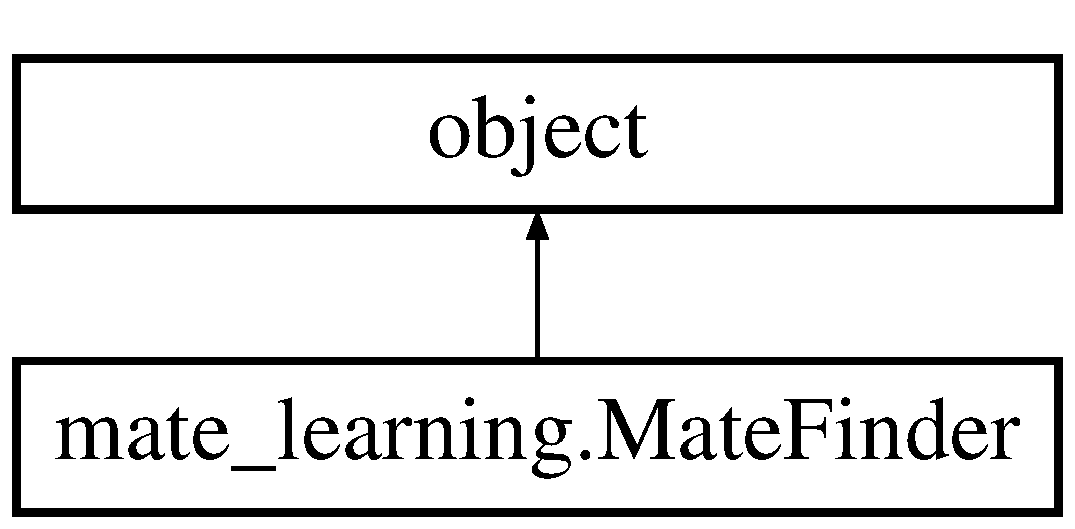
\includegraphics[height=2.000000cm]{classmate__learning_1_1_mate_finder}
\end{center}
\end{figure}
\subsection*{Public Member Functions}
\begin{DoxyCompactItemize}
\item 
def \hyperlink{classmate__learning_1_1_mate_finder_adb527f8a50802bee9dc7b976e38809bb}{\+\_\+\+\_\+init\+\_\+\+\_\+}
\begin{DoxyCompactList}\small\item\em Constructor for the Pair\+Finder object out of the given data set. \end{DoxyCompactList}\item 
def \hyperlink{classmate__learning_1_1_mate_finder_ad550cd77ba9a781f7eb09316de71f3f2}{validate\+\_\+groupings}
\begin{DoxyCompactList}\small\item\em It removes overlapping groupings (matings) among the list of groupings provided. \end{DoxyCompactList}\item 
def \hyperlink{classmate__learning_1_1_mate_finder_a45cb9b80fefff297b6c44a0d3bb81b83}{learn\+\_\+by\+\_\+mate\+\_\+discovery}
\begin{DoxyCompactList}\small\item\em Brute force discovery of mates and relevant components during the training phase so that accuracy is the highest among all possibilities. \end{DoxyCompactList}\item 
def \hyperlink{classmate__learning_1_1_mate_finder_ae5e19b18a5e29e8ada0303753f23aff0}{select\+\_\+\+K\+\_\+components}
\begin{DoxyCompactList}\small\item\em Find the k number of components that produce the highest prediction accuracy from the training procedure\+: \end{DoxyCompactList}\item 
def \hyperlink{classmate__learning_1_1_mate_finder_a2de3f01d6c2b6b73e8673abdd405b868}{get\+\_\+address}
\begin{DoxyCompactList}\small\item\em Resolves the address in the training L\+U\+T pertaining the given matings (a list of candidate matches) on the data set portion provided. \end{DoxyCompactList}\item 
def \hyperlink{classmate__learning_1_1_mate_finder_a096518e1bff5159c934c2e8affb5f40d}{get\+\_\+index\+\_\+address\+\_\+table}
\begin{DoxyCompactList}\small\item\em This is a vectorized function that resolves the index (a.\+k.\+a. \end{DoxyCompactList}\item 
def \hyperlink{classmate__learning_1_1_mate_finder_a6f3887d912b4f87eb612b6e67b38b8fd}{generate\+\_\+decision\+\_\+rules\+\_\+\+L\+U\+T}
\begin{DoxyCompactList}\small\item\em A decision rules are learned from the provided list of matings (non-\/overlapping groups) and the chosen components. \end{DoxyCompactList}\item 
def \hyperlink{classmate__learning_1_1_mate_finder_a79a1cb24bc6df0d732abd48b4ad0a63f}{compute\+\_\+prediction\+\_\+accuracy}
\begin{DoxyCompactList}\small\item\em The accuracy of correct classification using the provided decision rules is computed statistically. \end{DoxyCompactList}\item 
def \hyperlink{classmate__learning_1_1_mate_finder_aff6680733a2803e2e39f860fa63a0fd8}{predict\+\_\+category}
\begin{DoxyCompactList}\small\item\em With the given list of matings (groupings) and the decision rules table, the list of measurement vectors (instances) are classified accordingly. \end{DoxyCompactList}\end{DoxyCompactItemize}
\subsection*{Public Attributes}
\begin{DoxyCompactItemize}
\item 
\hyperlink{classmate__learning_1_1_mate_finder_a7347330ac72c85afd3f9fca87640d294}{all\+\_\+data}
\item 
\hyperlink{classmate__learning_1_1_mate_finder_a964c20920e14dfc4d5091142d429fe06}{all\+\_\+classes}
\item 
\hyperlink{classmate__learning_1_1_mate_finder_aeb435fdde37e9ac0cf72d03c25369201}{num\+\_\+of\+\_\+instances}
\item 
\hyperlink{classmate__learning_1_1_mate_finder_aaf6a72d379804901e89dc1c3e5ae5fd4}{num\+\_\+of\+\_\+components}
\item 
\hyperlink{classmate__learning_1_1_mate_finder_ad876941a4f4bf2e1dda05bf4881861e4}{num\+\_\+of\+\_\+values}
\item 
\hyperlink{classmate__learning_1_1_mate_finder_ac9e474a0c97351549960cd8baf0bbe24}{mating\+\_\+size}
\item 
\hyperlink{classmate__learning_1_1_mate_finder_a56553c3120e135bb4a969fd445f6bf6b}{num\+\_\+of\+\_\+mating\+\_\+groups}
\item 
\hyperlink{classmate__learning_1_1_mate_finder_af4f8fcfed10a8658bf2216f0deab368e}{map\+\_\+base}
\item 
\hyperlink{classmate__learning_1_1_mate_finder_a1d13f05feb21a3e48bf8822bf9c9fa67}{class\+\_\+learning}
\item 
\hyperlink{classmate__learning_1_1_mate_finder_a3fe8edaa8b6704d94252c2d1fc5b3360}{class\+\_\+test}
\item 
\hyperlink{classmate__learning_1_1_mate_finder_a04fe666220e1331ae3c444f3e8f6e3d3}{feat\+\_\+data\+\_\+learning\+\_\+train}
\item 
\hyperlink{classmate__learning_1_1_mate_finder_affd9b58edbaaa1e91f130ce9fcef958e}{class\+\_\+learning\+\_\+train}
\item 
\hyperlink{classmate__learning_1_1_mate_finder_a52a62e61246856c4d2e613a29ed86a8d}{feat\+\_\+data\+\_\+learning\+\_\+validate}
\item 
\hyperlink{classmate__learning_1_1_mate_finder_a958fd7ea70befe493a1d7f3d383d50c6}{class\+\_\+learning\+\_\+validate}
\item 
\hyperlink{classmate__learning_1_1_mate_finder_ad1790fa1f3465a0986165e11474723e2}{N\+\_\+train}
\item 
\hyperlink{classmate__learning_1_1_mate_finder_a6f92751c17d9794258343fd7c5d5a4d5}{c0\+\_\+indices\+\_\+train}
\item 
\hyperlink{classmate__learning_1_1_mate_finder_a247fd9ebecfbbcd44c638803cdaf2bce}{c1\+\_\+indices\+\_\+train}
\item 
\hyperlink{classmate__learning_1_1_mate_finder_a3577286991dc86227a3275cefd8d02af}{feat\+\_\+train\+\_\+c0}
\item 
\hyperlink{classmate__learning_1_1_mate_finder_a9c00a7acd25f415074e73b3d8862d38d}{feat\+\_\+train\+\_\+c1}
\item 
\hyperlink{classmate__learning_1_1_mate_finder_a72604851fbd5d9d64ef8f21ab3bbb08b}{values\+\_\+list}
\item 
\hyperlink{classmate__learning_1_1_mate_finder_a1feda94256f5a694c6102f83c3fc8ce7}{mates\+\_\+candidates\+\_\+per\+\_\+component}
\item 
\hyperlink{classmate__learning_1_1_mate_finder_ac42fe95eaa044c91077b75953128fc23}{address\+\_\+multiples}
\end{DoxyCompactItemize}
\subsection*{Private Member Functions}
\begin{DoxyCompactItemize}
\item 
def \hyperlink{classmate__learning_1_1_mate_finder_a43b8d42cc7b3529697262ad628c9cca9}{\+\_\+generate\+\_\+training\+\_\+\+L\+U\+T}
\begin{DoxyCompactList}\small\item\em Generates an empty look-\/up table that will be addressed to train the learned with the given data. \end{DoxyCompactList}\end{DoxyCompactItemize}


\subsection{Detailed Description}
Used for the particular binary classification problem based on mates (usually groups of 2 -\/ pairs) across each component of a discrete-\/valued data set. 

This class provides procedures such as the removal of irrelevant components (selection of relevant components), as well as essential learning (training and validation) and testing procedures from learned decision tables of pairs.

Once a \hyperlink{classmate__learning_1_1_mate_finder}{Mate\+Finder} object has been instantiated through the constructor, the interfacing methods employed by an external classifier are\+: \hyperlink{classmate__learning_1_1_mate_finder_a45cb9b80fefff297b6c44a0d3bb81b83}{learn\+\_\+by\+\_\+mate\+\_\+discovery()} and \hyperlink{classmate__learning_1_1_mate_finder_a79a1cb24bc6df0d732abd48b4ad0a63f}{compute\+\_\+prediction\+\_\+accuracy()} 

Definition at line 28 of file mate\+\_\+learning.\+py.



\subsection{Constructor \& Destructor Documentation}
\hypertarget{classmate__learning_1_1_mate_finder_adb527f8a50802bee9dc7b976e38809bb}{\index{mate\+\_\+learning\+::\+Mate\+Finder@{mate\+\_\+learning\+::\+Mate\+Finder}!\+\_\+\+\_\+init\+\_\+\+\_\+@{\+\_\+\+\_\+init\+\_\+\+\_\+}}
\index{\+\_\+\+\_\+init\+\_\+\+\_\+@{\+\_\+\+\_\+init\+\_\+\+\_\+}!mate\+\_\+learning\+::\+Mate\+Finder@{mate\+\_\+learning\+::\+Mate\+Finder}}
\subsubsection[{\+\_\+\+\_\+init\+\_\+\+\_\+}]{\setlength{\rightskip}{0pt plus 5cm}def mate\+\_\+learning.\+Mate\+Finder.\+\_\+\+\_\+init\+\_\+\+\_\+ (
\begin{DoxyParamCaption}
\item[{}]{self, }
\item[{}]{component\+\_\+data, }
\item[{}]{classification\+\_\+labels, }
\item[{}]{mating\+\_\+size = {\ttfamily 2}}
\end{DoxyParamCaption}
)}}\label{classmate__learning_1_1_mate_finder_adb527f8a50802bee9dc7b976e38809bb}


Constructor for the Pair\+Finder object out of the given data set. 

\+: The data set (and corresponing classification labels) are split into the following portions\+: 50\% for learning phase\+: 25\% training + 25\% validation 50\% for testing phase\+: the real test using the learned table of decision rules

This constructor initializes the reusable member variables that are called from other functions.


\begin{DoxyParams}{Parameters}
{\em component\+\_\+data} & A 2\+D matrix (numpy ndarray) of measurements (observations) to work with. A copy is created of this. \\
\hline
{\em classification\+\_\+labels} & The category classification\+\_\+labels as a 1\+D ndarray. Expected to be nonnegative integers \\
\hline
{\em mating\+\_\+size} & It should default to 2 (for pairs), but as in life, mating (a.\+k.\+a grouping) can be done using larger number of members. Note, the number of values (10 digits for this exercise) must be divisible by the mating\+\_\+size. For now, we basically can have only groups of 2 or 5. \\
\hline
\end{DoxyParams}


Definition at line 45 of file mate\+\_\+learning.\+py.



\subsection{Member Function Documentation}
\hypertarget{classmate__learning_1_1_mate_finder_a43b8d42cc7b3529697262ad628c9cca9}{\index{mate\+\_\+learning\+::\+Mate\+Finder@{mate\+\_\+learning\+::\+Mate\+Finder}!\+\_\+generate\+\_\+training\+\_\+\+L\+U\+T@{\+\_\+generate\+\_\+training\+\_\+\+L\+U\+T}}
\index{\+\_\+generate\+\_\+training\+\_\+\+L\+U\+T@{\+\_\+generate\+\_\+training\+\_\+\+L\+U\+T}!mate\+\_\+learning\+::\+Mate\+Finder@{mate\+\_\+learning\+::\+Mate\+Finder}}
\subsubsection[{\+\_\+generate\+\_\+training\+\_\+\+L\+U\+T}]{\setlength{\rightskip}{0pt plus 5cm}def mate\+\_\+learning.\+Mate\+Finder.\+\_\+generate\+\_\+training\+\_\+\+L\+U\+T (
\begin{DoxyParamCaption}
\item[{}]{self, }
\item[{}]{cols}
\end{DoxyParamCaption}
)\hspace{0.3cm}{\ttfamily [private]}}}\label{classmate__learning_1_1_mate_finder_a43b8d42cc7b3529697262ad628c9cca9}


Generates an empty look-\/up table that will be addressed to train the learned with the given data. 


\begin{DoxyParams}{Parameters}
{\em cols} & the number of columns (components) in the data set that are being used for the training.\\
\hline
\end{DoxyParams}
\begin{DoxyReturn}{Returns}
\+: An empty 2-\/dimensional matrix that can be addressed while performing decision statistics 
\end{DoxyReturn}


Definition at line 201 of file mate\+\_\+learning.\+py.



References mate\+\_\+learning.\+Mate\+Finder.\+num\+\_\+of\+\_\+mating\+\_\+groups.



Referenced by mate\+\_\+learning.\+Mate\+Finder.\+generate\+\_\+decision\+\_\+rules\+\_\+\+L\+U\+T().

\hypertarget{classmate__learning_1_1_mate_finder_a79a1cb24bc6df0d732abd48b4ad0a63f}{\index{mate\+\_\+learning\+::\+Mate\+Finder@{mate\+\_\+learning\+::\+Mate\+Finder}!compute\+\_\+prediction\+\_\+accuracy@{compute\+\_\+prediction\+\_\+accuracy}}
\index{compute\+\_\+prediction\+\_\+accuracy@{compute\+\_\+prediction\+\_\+accuracy}!mate\+\_\+learning\+::\+Mate\+Finder@{mate\+\_\+learning\+::\+Mate\+Finder}}
\subsubsection[{compute\+\_\+prediction\+\_\+accuracy}]{\setlength{\rightskip}{0pt plus 5cm}def mate\+\_\+learning.\+Mate\+Finder.\+compute\+\_\+prediction\+\_\+accuracy (
\begin{DoxyParamCaption}
\item[{}]{self, }
\item[{}]{matings, }
\item[{}]{decisions\+\_\+\+L\+U\+T, }
\item[{}]{relevant\+\_\+components = {\ttfamily None}, }
\item[{}]{comp\+\_\+data\+\_\+test = {\ttfamily None}, }
\item[{}]{class\+\_\+test = {\ttfamily None}, }
\item[{}]{verbose = {\ttfamily False}}
\end{DoxyParamCaption}
)}}\label{classmate__learning_1_1_mate_finder_a79a1cb24bc6df0d732abd48b4ad0a63f}


The accuracy of correct classification using the provided decision rules is computed statistically. 


\begin{DoxyParams}{Parameters}
{\em matings} & An ordered list of indices used to group employing the map\+\_\+based of choice set in the constructor. By default, the mapping is pair-\/wise ordered from left to right. \\
\hline
{\em decisions\+\_\+\+L\+U\+T} & The learned rules in a L\+U\+T \\
\hline
{\em relevant\+\_\+components} & By default is set to None, so all components will be used. Otherwise, this specifies the selection of components to work with. \\
\hline
{\em comp\+\_\+data\+\_\+test} & If any, this is the component data set to use for predicting upon and testing the classification accuracy with the provided matings and decision rules. Otherwise, it defaults to using the test data set (the 50\% of the entire data set passed in the constructor) \\
\hline
{\em class\+\_\+test} & The classification labels associated with comp\+\_\+data\+\_\+test if any. \\
\hline
{\em verbose} & Indicates whether to enable message verbosity.\\
\hline
\end{DoxyParams}
\begin{DoxyReturn}{Returns}
\+: The normalized accuracy of correct classification computed according to the specified parameters. 
\end{DoxyReturn}


Definition at line 293 of file mate\+\_\+learning.\+py.



References mate\+\_\+learning.\+Mate\+Finder.\+class\+\_\+test, and mate\+\_\+learning.\+Mate\+Finder.\+predict\+\_\+category().



Referenced by mate\+\_\+learning.\+Mate\+Finder.\+select\+\_\+\+K\+\_\+components().

\hypertarget{classmate__learning_1_1_mate_finder_a6f3887d912b4f87eb612b6e67b38b8fd}{\index{mate\+\_\+learning\+::\+Mate\+Finder@{mate\+\_\+learning\+::\+Mate\+Finder}!generate\+\_\+decision\+\_\+rules\+\_\+\+L\+U\+T@{generate\+\_\+decision\+\_\+rules\+\_\+\+L\+U\+T}}
\index{generate\+\_\+decision\+\_\+rules\+\_\+\+L\+U\+T@{generate\+\_\+decision\+\_\+rules\+\_\+\+L\+U\+T}!mate\+\_\+learning\+::\+Mate\+Finder@{mate\+\_\+learning\+::\+Mate\+Finder}}
\subsubsection[{generate\+\_\+decision\+\_\+rules\+\_\+\+L\+U\+T}]{\setlength{\rightskip}{0pt plus 5cm}def mate\+\_\+learning.\+Mate\+Finder.\+generate\+\_\+decision\+\_\+rules\+\_\+\+L\+U\+T (
\begin{DoxyParamCaption}
\item[{}]{self, }
\item[{}]{matings, }
\item[{}]{comp\+\_\+subset}
\end{DoxyParamCaption}
)}}\label{classmate__learning_1_1_mate_finder_a6f3887d912b4f87eb612b6e67b38b8fd}


A decision rules are learned from the provided list of matings (non-\/overlapping groups) and the chosen components. 


\begin{DoxyParams}{Parameters}
{\em matings} & An ordered list of indices used to group employing the map\+\_\+based of choice set in the constructor. By default, the mapping is pair-\/wise ordered from left to right. \\
\hline
{\em comp\+\_\+subset} & The list of selected component indices upon where the decision table is generated\\
\hline
\end{DoxyParams}
\begin{DoxyReturn}{Returns}
\+: The 1-\/\+D table of decision rules extracted from frequency analysis out of the learning portion of the data set 
\end{DoxyReturn}


Definition at line 255 of file mate\+\_\+learning.\+py.



References mate\+\_\+learning.\+Mate\+Finder.\+\_\+generate\+\_\+training\+\_\+\+L\+U\+T(), mate\+\_\+learning.\+Mate\+Finder.\+feat\+\_\+train\+\_\+c0, mate\+\_\+learning.\+Mate\+Finder.\+feat\+\_\+train\+\_\+c1, mate\+\_\+learning.\+Mate\+Finder.\+get\+\_\+address(), mate\+\_\+learning.\+Mate\+Finder.\+get\+\_\+index\+\_\+address\+\_\+table(), and mate\+\_\+learning.\+Mate\+Finder.\+N\+\_\+train.



Referenced by mate\+\_\+learning.\+Mate\+Finder.\+learn\+\_\+by\+\_\+mate\+\_\+discovery(), and mate\+\_\+learning.\+Mate\+Finder.\+select\+\_\+\+K\+\_\+components().

\hypertarget{classmate__learning_1_1_mate_finder_a2de3f01d6c2b6b73e8673abdd405b868}{\index{mate\+\_\+learning\+::\+Mate\+Finder@{mate\+\_\+learning\+::\+Mate\+Finder}!get\+\_\+address@{get\+\_\+address}}
\index{get\+\_\+address@{get\+\_\+address}!mate\+\_\+learning\+::\+Mate\+Finder@{mate\+\_\+learning\+::\+Mate\+Finder}}
\subsubsection[{get\+\_\+address}]{\setlength{\rightskip}{0pt plus 5cm}def mate\+\_\+learning.\+Mate\+Finder.\+get\+\_\+address (
\begin{DoxyParamCaption}
\item[{}]{self, }
\item[{}]{matings, }
\item[{}]{component\+\_\+data}
\end{DoxyParamCaption}
)}}\label{classmate__learning_1_1_mate_finder_a2de3f01d6c2b6b73e8673abdd405b868}


Resolves the address in the training L\+U\+T pertaining the given matings (a list of candidate matches) on the data set portion provided. 


\begin{DoxyParams}{Parameters}
{\em matings} & List of indices associated with the groupings (matches) \\
\hline
{\em component\+\_\+data} & The ndarray of component data for which addresses are resolved for\\
\hline
\end{DoxyParams}
\begin{DoxyReturn}{Returns}
\+: the numpy n-\/dimensional array of resolved addresses for the provided data and desired matings 
\end{DoxyReturn}


Definition at line 215 of file mate\+\_\+learning.\+py.



References mate\+\_\+learning.\+Mate\+Finder.\+map\+\_\+base, and mate\+\_\+learning.\+Mate\+Finder.\+values\+\_\+list.



Referenced by mate\+\_\+learning.\+Mate\+Finder.\+generate\+\_\+decision\+\_\+rules\+\_\+\+L\+U\+T(), and mate\+\_\+learning.\+Mate\+Finder.\+predict\+\_\+category().

\hypertarget{classmate__learning_1_1_mate_finder_a096518e1bff5159c934c2e8affb5f40d}{\index{mate\+\_\+learning\+::\+Mate\+Finder@{mate\+\_\+learning\+::\+Mate\+Finder}!get\+\_\+index\+\_\+address\+\_\+table@{get\+\_\+index\+\_\+address\+\_\+table}}
\index{get\+\_\+index\+\_\+address\+\_\+table@{get\+\_\+index\+\_\+address\+\_\+table}!mate\+\_\+learning\+::\+Mate\+Finder@{mate\+\_\+learning\+::\+Mate\+Finder}}
\subsubsection[{get\+\_\+index\+\_\+address\+\_\+table}]{\setlength{\rightskip}{0pt plus 5cm}def mate\+\_\+learning.\+Mate\+Finder.\+get\+\_\+index\+\_\+address\+\_\+table (
\begin{DoxyParamCaption}
\item[{}]{self, }
\item[{}]{address}
\end{DoxyParamCaption}
)}}\label{classmate__learning_1_1_mate_finder_a096518e1bff5159c934c2e8affb5f40d}


This is a vectorized function that resolves the index (a.\+k.\+a. 

hash address) on the 1-\/\+D array of rules employing in the learning/testing procedure).


\begin{DoxyParams}{Parameters}
{\em address} & An array of address arrays to be hashed for on a 1-\/\+D table using the pertaining base (such as base 5 when dealing with groups of 2)\\
\hline
\end{DoxyParams}
\begin{DoxyReturn}{Returns}
\+: the resolved 1-\/\+D array of indices corresponding the input address. 
\end{DoxyReturn}


Definition at line 241 of file mate\+\_\+learning.\+py.



References mate\+\_\+learning.\+Mate\+Finder.\+address\+\_\+multiples.



Referenced by mate\+\_\+learning.\+Mate\+Finder.\+generate\+\_\+decision\+\_\+rules\+\_\+\+L\+U\+T(), and mate\+\_\+learning.\+Mate\+Finder.\+predict\+\_\+category().

\hypertarget{classmate__learning_1_1_mate_finder_a45cb9b80fefff297b6c44a0d3bb81b83}{\index{mate\+\_\+learning\+::\+Mate\+Finder@{mate\+\_\+learning\+::\+Mate\+Finder}!learn\+\_\+by\+\_\+mate\+\_\+discovery@{learn\+\_\+by\+\_\+mate\+\_\+discovery}}
\index{learn\+\_\+by\+\_\+mate\+\_\+discovery@{learn\+\_\+by\+\_\+mate\+\_\+discovery}!mate\+\_\+learning\+::\+Mate\+Finder@{mate\+\_\+learning\+::\+Mate\+Finder}}
\subsubsection[{learn\+\_\+by\+\_\+mate\+\_\+discovery}]{\setlength{\rightskip}{0pt plus 5cm}def mate\+\_\+learning.\+Mate\+Finder.\+learn\+\_\+by\+\_\+mate\+\_\+discovery (
\begin{DoxyParamCaption}
\item[{}]{self}
\end{DoxyParamCaption}
)}}\label{classmate__learning_1_1_mate_finder_a45cb9b80fefff297b6c44a0d3bb81b83}


Brute force discovery of mates and relevant components during the training phase so that accuracy is the highest among all possibilities. 

\begin{DoxyReturn}{Returns}
The 1-\/d numpy array (table) of learned rules. 

List of best combination of mates (pairs) across the discovered relevant components 

The list of discovered relevant components from the training phase 
\end{DoxyReturn}


Definition at line 120 of file mate\+\_\+learning.\+py.



References mate\+\_\+learning.\+Mate\+Finder.\+generate\+\_\+decision\+\_\+rules\+\_\+\+L\+U\+T(), mate\+\_\+learning.\+Mate\+Finder.\+num\+\_\+of\+\_\+components, and mate\+\_\+learning.\+Mate\+Finder.\+select\+\_\+\+K\+\_\+components().

\hypertarget{classmate__learning_1_1_mate_finder_aff6680733a2803e2e39f860fa63a0fd8}{\index{mate\+\_\+learning\+::\+Mate\+Finder@{mate\+\_\+learning\+::\+Mate\+Finder}!predict\+\_\+category@{predict\+\_\+category}}
\index{predict\+\_\+category@{predict\+\_\+category}!mate\+\_\+learning\+::\+Mate\+Finder@{mate\+\_\+learning\+::\+Mate\+Finder}}
\subsubsection[{predict\+\_\+category}]{\setlength{\rightskip}{0pt plus 5cm}def mate\+\_\+learning.\+Mate\+Finder.\+predict\+\_\+category (
\begin{DoxyParamCaption}
\item[{}]{self, }
\item[{}]{matings, }
\item[{}]{decisions\+\_\+\+L\+U\+T, }
\item[{}]{instance\+\_\+vector}
\end{DoxyParamCaption}
)}}\label{classmate__learning_1_1_mate_finder_aff6680733a2803e2e39f860fa63a0fd8}


With the given list of matings (groupings) and the decision rules table, the list of measurement vectors (instances) are classified accordingly. 


\begin{DoxyParams}{Parameters}
{\em matings} & An ordered list of indices used to group employing the map\+\_\+based of choice set in the constructor. By default, the mapping is pair-\/wise ordered from left to right. \\
\hline
{\em decisions\+\_\+\+L\+U\+T} & The learned rules in a L\+U\+T \\
\hline
{\em instance\+\_\+vector} & The list of measurement vectors (instances, a.\+k.\+a observations) to classify.\\
\hline
\end{DoxyParams}
\begin{DoxyReturn}{Returns}
\+: The classification results corresponding to the supplied instance vectors for the specified rules and matings. 
\end{DoxyReturn}


Definition at line 325 of file mate\+\_\+learning.\+py.



References mate\+\_\+learning.\+Mate\+Finder.\+get\+\_\+address(), and mate\+\_\+learning.\+Mate\+Finder.\+get\+\_\+index\+\_\+address\+\_\+table().



Referenced by mate\+\_\+learning.\+Mate\+Finder.\+compute\+\_\+prediction\+\_\+accuracy().

\hypertarget{classmate__learning_1_1_mate_finder_ae5e19b18a5e29e8ada0303753f23aff0}{\index{mate\+\_\+learning\+::\+Mate\+Finder@{mate\+\_\+learning\+::\+Mate\+Finder}!select\+\_\+\+K\+\_\+components@{select\+\_\+\+K\+\_\+components}}
\index{select\+\_\+\+K\+\_\+components@{select\+\_\+\+K\+\_\+components}!mate\+\_\+learning\+::\+Mate\+Finder@{mate\+\_\+learning\+::\+Mate\+Finder}}
\subsubsection[{select\+\_\+\+K\+\_\+components}]{\setlength{\rightskip}{0pt plus 5cm}def mate\+\_\+learning.\+Mate\+Finder.\+select\+\_\+\+K\+\_\+components (
\begin{DoxyParamCaption}
\item[{}]{self, }
\item[{}]{k\+\_\+comps, }
\item[{}]{verbose = {\ttfamily True}}
\end{DoxyParamCaption}
)}}\label{classmate__learning_1_1_mate_finder_ae5e19b18a5e29e8ada0303753f23aff0}


Find the k number of components that produce the highest prediction accuracy from the training procedure\+: 

Learning of rules is performed on the training portion of the data set (technically, the 25\% of the entire data set) Accuracy validation to choose best is performed on the validation data set (technically, the other 25\% of the entire data set)


\begin{DoxyParams}{Parameters}
{\em k\+\_\+comps} & Indicates the number of components to be attempted the \char`\"{}brute-\/force\char`\"{} search upon.\\
\hline
\end{DoxyParams}
\begin{DoxyReturn}{Returns}
The accuracy (normalized value from 0 to 1.\+0) obtained using the best selection of k components 

List of best combination of mates (pairs) across the best selected components 

The list of the best selected components 
\end{DoxyReturn}


Definition at line 160 of file mate\+\_\+learning.\+py.



References mate\+\_\+learning.\+Mate\+Finder.\+class\+\_\+learning\+\_\+validate, mate\+\_\+learning.\+Mate\+Finder.\+compute\+\_\+prediction\+\_\+accuracy(), mate\+\_\+learning.\+Mate\+Finder.\+feat\+\_\+data\+\_\+learning\+\_\+validate, mate\+\_\+learning.\+Mate\+Finder.\+generate\+\_\+decision\+\_\+rules\+\_\+\+L\+U\+T(), mate\+\_\+learning.\+Mate\+Finder.\+mates\+\_\+candidates\+\_\+per\+\_\+component, and mate\+\_\+learning.\+Mate\+Finder.\+num\+\_\+of\+\_\+components.



Referenced by mate\+\_\+learning.\+Mate\+Finder.\+learn\+\_\+by\+\_\+mate\+\_\+discovery().

\hypertarget{classmate__learning_1_1_mate_finder_ad550cd77ba9a781f7eb09316de71f3f2}{\index{mate\+\_\+learning\+::\+Mate\+Finder@{mate\+\_\+learning\+::\+Mate\+Finder}!validate\+\_\+groupings@{validate\+\_\+groupings}}
\index{validate\+\_\+groupings@{validate\+\_\+groupings}!mate\+\_\+learning\+::\+Mate\+Finder@{mate\+\_\+learning\+::\+Mate\+Finder}}
\subsubsection[{validate\+\_\+groupings}]{\setlength{\rightskip}{0pt plus 5cm}def mate\+\_\+learning.\+Mate\+Finder.\+validate\+\_\+groupings (
\begin{DoxyParamCaption}
\item[{}]{self, }
\item[{}]{candidate\+\_\+lists}
\end{DoxyParamCaption}
)}}\label{classmate__learning_1_1_mate_finder_ad550cd77ba9a781f7eb09316de71f3f2}


It removes overlapping groupings (matings) among the list of groupings provided. 


\begin{DoxyParams}{Parameters}
{\em candidate\+\_\+lists} & An ndarray of all possible groupings (in our particular exercise, these are all possible combinations of 2 out of 10 digits)\\
\hline
\end{DoxyParams}
\begin{DoxyReturn}{Returns}
\+: the filtered list of non-\/overlapping groupings. The reduction in length for this list is crucial for faster results during learning procedure. 
\end{DoxyReturn}


Definition at line 96 of file mate\+\_\+learning.\+py.



\subsection{Member Data Documentation}
\hypertarget{classmate__learning_1_1_mate_finder_ac42fe95eaa044c91077b75953128fc23}{\index{mate\+\_\+learning\+::\+Mate\+Finder@{mate\+\_\+learning\+::\+Mate\+Finder}!address\+\_\+multiples@{address\+\_\+multiples}}
\index{address\+\_\+multiples@{address\+\_\+multiples}!mate\+\_\+learning\+::\+Mate\+Finder@{mate\+\_\+learning\+::\+Mate\+Finder}}
\subsubsection[{address\+\_\+multiples}]{\setlength{\rightskip}{0pt plus 5cm}mate\+\_\+learning.\+Mate\+Finder.\+address\+\_\+multiples}}\label{classmate__learning_1_1_mate_finder_ac42fe95eaa044c91077b75953128fc23}


Definition at line 85 of file mate\+\_\+learning.\+py.



Referenced by mate\+\_\+learning.\+Mate\+Finder.\+get\+\_\+index\+\_\+address\+\_\+table().

\hypertarget{classmate__learning_1_1_mate_finder_a964c20920e14dfc4d5091142d429fe06}{\index{mate\+\_\+learning\+::\+Mate\+Finder@{mate\+\_\+learning\+::\+Mate\+Finder}!all\+\_\+classes@{all\+\_\+classes}}
\index{all\+\_\+classes@{all\+\_\+classes}!mate\+\_\+learning\+::\+Mate\+Finder@{mate\+\_\+learning\+::\+Mate\+Finder}}
\subsubsection[{all\+\_\+classes}]{\setlength{\rightskip}{0pt plus 5cm}mate\+\_\+learning.\+Mate\+Finder.\+all\+\_\+classes}}\label{classmate__learning_1_1_mate_finder_a964c20920e14dfc4d5091142d429fe06}


Definition at line 48 of file mate\+\_\+learning.\+py.

\hypertarget{classmate__learning_1_1_mate_finder_a7347330ac72c85afd3f9fca87640d294}{\index{mate\+\_\+learning\+::\+Mate\+Finder@{mate\+\_\+learning\+::\+Mate\+Finder}!all\+\_\+data@{all\+\_\+data}}
\index{all\+\_\+data@{all\+\_\+data}!mate\+\_\+learning\+::\+Mate\+Finder@{mate\+\_\+learning\+::\+Mate\+Finder}}
\subsubsection[{all\+\_\+data}]{\setlength{\rightskip}{0pt plus 5cm}mate\+\_\+learning.\+Mate\+Finder.\+all\+\_\+data}}\label{classmate__learning_1_1_mate_finder_a7347330ac72c85afd3f9fca87640d294}


Definition at line 47 of file mate\+\_\+learning.\+py.

\hypertarget{classmate__learning_1_1_mate_finder_a6f92751c17d9794258343fd7c5d5a4d5}{\index{mate\+\_\+learning\+::\+Mate\+Finder@{mate\+\_\+learning\+::\+Mate\+Finder}!c0\+\_\+indices\+\_\+train@{c0\+\_\+indices\+\_\+train}}
\index{c0\+\_\+indices\+\_\+train@{c0\+\_\+indices\+\_\+train}!mate\+\_\+learning\+::\+Mate\+Finder@{mate\+\_\+learning\+::\+Mate\+Finder}}
\subsubsection[{c0\+\_\+indices\+\_\+train}]{\setlength{\rightskip}{0pt plus 5cm}mate\+\_\+learning.\+Mate\+Finder.\+c0\+\_\+indices\+\_\+train}}\label{classmate__learning_1_1_mate_finder_a6f92751c17d9794258343fd7c5d5a4d5}


Definition at line 70 of file mate\+\_\+learning.\+py.

\hypertarget{classmate__learning_1_1_mate_finder_a247fd9ebecfbbcd44c638803cdaf2bce}{\index{mate\+\_\+learning\+::\+Mate\+Finder@{mate\+\_\+learning\+::\+Mate\+Finder}!c1\+\_\+indices\+\_\+train@{c1\+\_\+indices\+\_\+train}}
\index{c1\+\_\+indices\+\_\+train@{c1\+\_\+indices\+\_\+train}!mate\+\_\+learning\+::\+Mate\+Finder@{mate\+\_\+learning\+::\+Mate\+Finder}}
\subsubsection[{c1\+\_\+indices\+\_\+train}]{\setlength{\rightskip}{0pt plus 5cm}mate\+\_\+learning.\+Mate\+Finder.\+c1\+\_\+indices\+\_\+train}}\label{classmate__learning_1_1_mate_finder_a247fd9ebecfbbcd44c638803cdaf2bce}


Definition at line 71 of file mate\+\_\+learning.\+py.

\hypertarget{classmate__learning_1_1_mate_finder_a1d13f05feb21a3e48bf8822bf9c9fa67}{\index{mate\+\_\+learning\+::\+Mate\+Finder@{mate\+\_\+learning\+::\+Mate\+Finder}!class\+\_\+learning@{class\+\_\+learning}}
\index{class\+\_\+learning@{class\+\_\+learning}!mate\+\_\+learning\+::\+Mate\+Finder@{mate\+\_\+learning\+::\+Mate\+Finder}}
\subsubsection[{class\+\_\+learning}]{\setlength{\rightskip}{0pt plus 5cm}mate\+\_\+learning.\+Mate\+Finder.\+class\+\_\+learning}}\label{classmate__learning_1_1_mate_finder_a1d13f05feb21a3e48bf8822bf9c9fa67}


Definition at line 59 of file mate\+\_\+learning.\+py.

\hypertarget{classmate__learning_1_1_mate_finder_affd9b58edbaaa1e91f130ce9fcef958e}{\index{mate\+\_\+learning\+::\+Mate\+Finder@{mate\+\_\+learning\+::\+Mate\+Finder}!class\+\_\+learning\+\_\+train@{class\+\_\+learning\+\_\+train}}
\index{class\+\_\+learning\+\_\+train@{class\+\_\+learning\+\_\+train}!mate\+\_\+learning\+::\+Mate\+Finder@{mate\+\_\+learning\+::\+Mate\+Finder}}
\subsubsection[{class\+\_\+learning\+\_\+train}]{\setlength{\rightskip}{0pt plus 5cm}mate\+\_\+learning.\+Mate\+Finder.\+class\+\_\+learning\+\_\+train}}\label{classmate__learning_1_1_mate_finder_affd9b58edbaaa1e91f130ce9fcef958e}


Definition at line 64 of file mate\+\_\+learning.\+py.

\hypertarget{classmate__learning_1_1_mate_finder_a958fd7ea70befe493a1d7f3d383d50c6}{\index{mate\+\_\+learning\+::\+Mate\+Finder@{mate\+\_\+learning\+::\+Mate\+Finder}!class\+\_\+learning\+\_\+validate@{class\+\_\+learning\+\_\+validate}}
\index{class\+\_\+learning\+\_\+validate@{class\+\_\+learning\+\_\+validate}!mate\+\_\+learning\+::\+Mate\+Finder@{mate\+\_\+learning\+::\+Mate\+Finder}}
\subsubsection[{class\+\_\+learning\+\_\+validate}]{\setlength{\rightskip}{0pt plus 5cm}mate\+\_\+learning.\+Mate\+Finder.\+class\+\_\+learning\+\_\+validate}}\label{classmate__learning_1_1_mate_finder_a958fd7ea70befe493a1d7f3d383d50c6}


Definition at line 66 of file mate\+\_\+learning.\+py.



Referenced by mate\+\_\+learning.\+Mate\+Finder.\+select\+\_\+\+K\+\_\+components().

\hypertarget{classmate__learning_1_1_mate_finder_a3fe8edaa8b6704d94252c2d1fc5b3360}{\index{mate\+\_\+learning\+::\+Mate\+Finder@{mate\+\_\+learning\+::\+Mate\+Finder}!class\+\_\+test@{class\+\_\+test}}
\index{class\+\_\+test@{class\+\_\+test}!mate\+\_\+learning\+::\+Mate\+Finder@{mate\+\_\+learning\+::\+Mate\+Finder}}
\subsubsection[{class\+\_\+test}]{\setlength{\rightskip}{0pt plus 5cm}mate\+\_\+learning.\+Mate\+Finder.\+class\+\_\+test}}\label{classmate__learning_1_1_mate_finder_a3fe8edaa8b6704d94252c2d1fc5b3360}


Definition at line 60 of file mate\+\_\+learning.\+py.



Referenced by mate\+\_\+learning.\+Mate\+Finder.\+compute\+\_\+prediction\+\_\+accuracy().

\hypertarget{classmate__learning_1_1_mate_finder_a04fe666220e1331ae3c444f3e8f6e3d3}{\index{mate\+\_\+learning\+::\+Mate\+Finder@{mate\+\_\+learning\+::\+Mate\+Finder}!feat\+\_\+data\+\_\+learning\+\_\+train@{feat\+\_\+data\+\_\+learning\+\_\+train}}
\index{feat\+\_\+data\+\_\+learning\+\_\+train@{feat\+\_\+data\+\_\+learning\+\_\+train}!mate\+\_\+learning\+::\+Mate\+Finder@{mate\+\_\+learning\+::\+Mate\+Finder}}
\subsubsection[{feat\+\_\+data\+\_\+learning\+\_\+train}]{\setlength{\rightskip}{0pt plus 5cm}mate\+\_\+learning.\+Mate\+Finder.\+feat\+\_\+data\+\_\+learning\+\_\+train}}\label{classmate__learning_1_1_mate_finder_a04fe666220e1331ae3c444f3e8f6e3d3}


Definition at line 63 of file mate\+\_\+learning.\+py.

\hypertarget{classmate__learning_1_1_mate_finder_a52a62e61246856c4d2e613a29ed86a8d}{\index{mate\+\_\+learning\+::\+Mate\+Finder@{mate\+\_\+learning\+::\+Mate\+Finder}!feat\+\_\+data\+\_\+learning\+\_\+validate@{feat\+\_\+data\+\_\+learning\+\_\+validate}}
\index{feat\+\_\+data\+\_\+learning\+\_\+validate@{feat\+\_\+data\+\_\+learning\+\_\+validate}!mate\+\_\+learning\+::\+Mate\+Finder@{mate\+\_\+learning\+::\+Mate\+Finder}}
\subsubsection[{feat\+\_\+data\+\_\+learning\+\_\+validate}]{\setlength{\rightskip}{0pt plus 5cm}mate\+\_\+learning.\+Mate\+Finder.\+feat\+\_\+data\+\_\+learning\+\_\+validate}}\label{classmate__learning_1_1_mate_finder_a52a62e61246856c4d2e613a29ed86a8d}


Definition at line 65 of file mate\+\_\+learning.\+py.



Referenced by mate\+\_\+learning.\+Mate\+Finder.\+select\+\_\+\+K\+\_\+components().

\hypertarget{classmate__learning_1_1_mate_finder_a3577286991dc86227a3275cefd8d02af}{\index{mate\+\_\+learning\+::\+Mate\+Finder@{mate\+\_\+learning\+::\+Mate\+Finder}!feat\+\_\+train\+\_\+c0@{feat\+\_\+train\+\_\+c0}}
\index{feat\+\_\+train\+\_\+c0@{feat\+\_\+train\+\_\+c0}!mate\+\_\+learning\+::\+Mate\+Finder@{mate\+\_\+learning\+::\+Mate\+Finder}}
\subsubsection[{feat\+\_\+train\+\_\+c0}]{\setlength{\rightskip}{0pt plus 5cm}mate\+\_\+learning.\+Mate\+Finder.\+feat\+\_\+train\+\_\+c0}}\label{classmate__learning_1_1_mate_finder_a3577286991dc86227a3275cefd8d02af}


Definition at line 72 of file mate\+\_\+learning.\+py.



Referenced by mate\+\_\+learning.\+Mate\+Finder.\+generate\+\_\+decision\+\_\+rules\+\_\+\+L\+U\+T().

\hypertarget{classmate__learning_1_1_mate_finder_a9c00a7acd25f415074e73b3d8862d38d}{\index{mate\+\_\+learning\+::\+Mate\+Finder@{mate\+\_\+learning\+::\+Mate\+Finder}!feat\+\_\+train\+\_\+c1@{feat\+\_\+train\+\_\+c1}}
\index{feat\+\_\+train\+\_\+c1@{feat\+\_\+train\+\_\+c1}!mate\+\_\+learning\+::\+Mate\+Finder@{mate\+\_\+learning\+::\+Mate\+Finder}}
\subsubsection[{feat\+\_\+train\+\_\+c1}]{\setlength{\rightskip}{0pt plus 5cm}mate\+\_\+learning.\+Mate\+Finder.\+feat\+\_\+train\+\_\+c1}}\label{classmate__learning_1_1_mate_finder_a9c00a7acd25f415074e73b3d8862d38d}


Definition at line 73 of file mate\+\_\+learning.\+py.



Referenced by mate\+\_\+learning.\+Mate\+Finder.\+generate\+\_\+decision\+\_\+rules\+\_\+\+L\+U\+T().

\hypertarget{classmate__learning_1_1_mate_finder_af4f8fcfed10a8658bf2216f0deab368e}{\index{mate\+\_\+learning\+::\+Mate\+Finder@{mate\+\_\+learning\+::\+Mate\+Finder}!map\+\_\+base@{map\+\_\+base}}
\index{map\+\_\+base@{map\+\_\+base}!mate\+\_\+learning\+::\+Mate\+Finder@{mate\+\_\+learning\+::\+Mate\+Finder}}
\subsubsection[{map\+\_\+base}]{\setlength{\rightskip}{0pt plus 5cm}mate\+\_\+learning.\+Mate\+Finder.\+map\+\_\+base}}\label{classmate__learning_1_1_mate_finder_af4f8fcfed10a8658bf2216f0deab368e}


Definition at line 54 of file mate\+\_\+learning.\+py.



Referenced by mate\+\_\+learning.\+Mate\+Finder.\+get\+\_\+address().

\hypertarget{classmate__learning_1_1_mate_finder_a1feda94256f5a694c6102f83c3fc8ce7}{\index{mate\+\_\+learning\+::\+Mate\+Finder@{mate\+\_\+learning\+::\+Mate\+Finder}!mates\+\_\+candidates\+\_\+per\+\_\+component@{mates\+\_\+candidates\+\_\+per\+\_\+component}}
\index{mates\+\_\+candidates\+\_\+per\+\_\+component@{mates\+\_\+candidates\+\_\+per\+\_\+component}!mate\+\_\+learning\+::\+Mate\+Finder@{mate\+\_\+learning\+::\+Mate\+Finder}}
\subsubsection[{mates\+\_\+candidates\+\_\+per\+\_\+component}]{\setlength{\rightskip}{0pt plus 5cm}mate\+\_\+learning.\+Mate\+Finder.\+mates\+\_\+candidates\+\_\+per\+\_\+component}}\label{classmate__learning_1_1_mate_finder_a1feda94256f5a694c6102f83c3fc8ce7}


Definition at line 82 of file mate\+\_\+learning.\+py.



Referenced by mate\+\_\+learning.\+Mate\+Finder.\+select\+\_\+\+K\+\_\+components().

\hypertarget{classmate__learning_1_1_mate_finder_ac9e474a0c97351549960cd8baf0bbe24}{\index{mate\+\_\+learning\+::\+Mate\+Finder@{mate\+\_\+learning\+::\+Mate\+Finder}!mating\+\_\+size@{mating\+\_\+size}}
\index{mating\+\_\+size@{mating\+\_\+size}!mate\+\_\+learning\+::\+Mate\+Finder@{mate\+\_\+learning\+::\+Mate\+Finder}}
\subsubsection[{mating\+\_\+size}]{\setlength{\rightskip}{0pt plus 5cm}mate\+\_\+learning.\+Mate\+Finder.\+mating\+\_\+size}}\label{classmate__learning_1_1_mate_finder_ac9e474a0c97351549960cd8baf0bbe24}


Definition at line 52 of file mate\+\_\+learning.\+py.

\hypertarget{classmate__learning_1_1_mate_finder_ad1790fa1f3465a0986165e11474723e2}{\index{mate\+\_\+learning\+::\+Mate\+Finder@{mate\+\_\+learning\+::\+Mate\+Finder}!N\+\_\+train@{N\+\_\+train}}
\index{N\+\_\+train@{N\+\_\+train}!mate\+\_\+learning\+::\+Mate\+Finder@{mate\+\_\+learning\+::\+Mate\+Finder}}
\subsubsection[{N\+\_\+train}]{\setlength{\rightskip}{0pt plus 5cm}mate\+\_\+learning.\+Mate\+Finder.\+N\+\_\+train}}\label{classmate__learning_1_1_mate_finder_ad1790fa1f3465a0986165e11474723e2}


Definition at line 67 of file mate\+\_\+learning.\+py.



Referenced by mate\+\_\+learning.\+Mate\+Finder.\+generate\+\_\+decision\+\_\+rules\+\_\+\+L\+U\+T().

\hypertarget{classmate__learning_1_1_mate_finder_aaf6a72d379804901e89dc1c3e5ae5fd4}{\index{mate\+\_\+learning\+::\+Mate\+Finder@{mate\+\_\+learning\+::\+Mate\+Finder}!num\+\_\+of\+\_\+components@{num\+\_\+of\+\_\+components}}
\index{num\+\_\+of\+\_\+components@{num\+\_\+of\+\_\+components}!mate\+\_\+learning\+::\+Mate\+Finder@{mate\+\_\+learning\+::\+Mate\+Finder}}
\subsubsection[{num\+\_\+of\+\_\+components}]{\setlength{\rightskip}{0pt plus 5cm}mate\+\_\+learning.\+Mate\+Finder.\+num\+\_\+of\+\_\+components}}\label{classmate__learning_1_1_mate_finder_aaf6a72d379804901e89dc1c3e5ae5fd4}


Definition at line 50 of file mate\+\_\+learning.\+py.



Referenced by mate\+\_\+learning.\+Mate\+Finder.\+learn\+\_\+by\+\_\+mate\+\_\+discovery(), and mate\+\_\+learning.\+Mate\+Finder.\+select\+\_\+\+K\+\_\+components().

\hypertarget{classmate__learning_1_1_mate_finder_aeb435fdde37e9ac0cf72d03c25369201}{\index{mate\+\_\+learning\+::\+Mate\+Finder@{mate\+\_\+learning\+::\+Mate\+Finder}!num\+\_\+of\+\_\+instances@{num\+\_\+of\+\_\+instances}}
\index{num\+\_\+of\+\_\+instances@{num\+\_\+of\+\_\+instances}!mate\+\_\+learning\+::\+Mate\+Finder@{mate\+\_\+learning\+::\+Mate\+Finder}}
\subsubsection[{num\+\_\+of\+\_\+instances}]{\setlength{\rightskip}{0pt plus 5cm}mate\+\_\+learning.\+Mate\+Finder.\+num\+\_\+of\+\_\+instances}}\label{classmate__learning_1_1_mate_finder_aeb435fdde37e9ac0cf72d03c25369201}


Definition at line 49 of file mate\+\_\+learning.\+py.

\hypertarget{classmate__learning_1_1_mate_finder_a56553c3120e135bb4a969fd445f6bf6b}{\index{mate\+\_\+learning\+::\+Mate\+Finder@{mate\+\_\+learning\+::\+Mate\+Finder}!num\+\_\+of\+\_\+mating\+\_\+groups@{num\+\_\+of\+\_\+mating\+\_\+groups}}
\index{num\+\_\+of\+\_\+mating\+\_\+groups@{num\+\_\+of\+\_\+mating\+\_\+groups}!mate\+\_\+learning\+::\+Mate\+Finder@{mate\+\_\+learning\+::\+Mate\+Finder}}
\subsubsection[{num\+\_\+of\+\_\+mating\+\_\+groups}]{\setlength{\rightskip}{0pt plus 5cm}mate\+\_\+learning.\+Mate\+Finder.\+num\+\_\+of\+\_\+mating\+\_\+groups}}\label{classmate__learning_1_1_mate_finder_a56553c3120e135bb4a969fd445f6bf6b}


Definition at line 53 of file mate\+\_\+learning.\+py.



Referenced by mate\+\_\+learning.\+Mate\+Finder.\+\_\+generate\+\_\+training\+\_\+\+L\+U\+T().

\hypertarget{classmate__learning_1_1_mate_finder_ad876941a4f4bf2e1dda05bf4881861e4}{\index{mate\+\_\+learning\+::\+Mate\+Finder@{mate\+\_\+learning\+::\+Mate\+Finder}!num\+\_\+of\+\_\+values@{num\+\_\+of\+\_\+values}}
\index{num\+\_\+of\+\_\+values@{num\+\_\+of\+\_\+values}!mate\+\_\+learning\+::\+Mate\+Finder@{mate\+\_\+learning\+::\+Mate\+Finder}}
\subsubsection[{num\+\_\+of\+\_\+values}]{\setlength{\rightskip}{0pt plus 5cm}mate\+\_\+learning.\+Mate\+Finder.\+num\+\_\+of\+\_\+values}}\label{classmate__learning_1_1_mate_finder_ad876941a4f4bf2e1dda05bf4881861e4}


Definition at line 51 of file mate\+\_\+learning.\+py.

\hypertarget{classmate__learning_1_1_mate_finder_a72604851fbd5d9d64ef8f21ab3bbb08b}{\index{mate\+\_\+learning\+::\+Mate\+Finder@{mate\+\_\+learning\+::\+Mate\+Finder}!values\+\_\+list@{values\+\_\+list}}
\index{values\+\_\+list@{values\+\_\+list}!mate\+\_\+learning\+::\+Mate\+Finder@{mate\+\_\+learning\+::\+Mate\+Finder}}
\subsubsection[{values\+\_\+list}]{\setlength{\rightskip}{0pt plus 5cm}mate\+\_\+learning.\+Mate\+Finder.\+values\+\_\+list}}\label{classmate__learning_1_1_mate_finder_a72604851fbd5d9d64ef8f21ab3bbb08b}


Definition at line 78 of file mate\+\_\+learning.\+py.



Referenced by mate\+\_\+learning.\+Mate\+Finder.\+get\+\_\+address().



The documentation for this class was generated from the following file\+:\begin{DoxyCompactItemize}
\item 
\hyperlink{mate__learning_8py}{mate\+\_\+learning.\+py}\end{DoxyCompactItemize}

\chapter{File Documentation}
\hypertarget{common__tools_8py}{\section{common\+\_\+tools.\+py File Reference}
\label{common__tools_8py}\index{common\+\_\+tools.\+py@{common\+\_\+tools.\+py}}
}
\subsection*{Namespaces}
\begin{DoxyCompactItemize}
\item 
 \hyperlink{namespacecommon__tools}{common\+\_\+tools}
\end{DoxyCompactItemize}
\subsection*{Functions}
\begin{DoxyCompactItemize}
\item 
def \hyperlink{namespacecommon__tools_a99127ed524481a987098d0b646248ac7}{common\+\_\+tools.\+get\+\_\+namestr}
\begin{DoxyCompactList}\small\item\em Finds and returns the variable name for the object instance in question in the desired namespace. \end{DoxyCompactList}\item 
def \hyperlink{namespacecommon__tools_a31bbee936ad9ee3f26d71ba58c435125}{common\+\_\+tools.\+save\+\_\+obj\+\_\+in\+\_\+pickle}
\item 
def \hyperlink{namespacecommon__tools_ae02aaf0ee60b16dd5d22f2e3f20fd9e6}{common\+\_\+tools.\+load\+\_\+obj\+\_\+from\+\_\+pickle}
\item 
def \hyperlink{namespacecommon__tools_ae5d41b7419e727e4389ae0a37f684a7f}{common\+\_\+tools.\+save\+\_\+dataset\+\_\+to\+\_\+pickle}
\item 
def \hyperlink{namespacecommon__tools_a38d5594d132460ab544508a860c74840}{common\+\_\+tools.\+load\+\_\+dataset\+\_\+from\+\_\+pickle}
\item 
def \hyperlink{namespacecommon__tools_a7987ebb2fe78986ee5bd276b9ca23b54}{common\+\_\+tools.\+read\+\_\+data}
\item 
def \hyperlink{namespacecommon__tools_aaa8d6759ce602c7555a4f247523a7b17}{common\+\_\+tools.\+filter\+\_\+irrelevant\+\_\+features}
\item 
def \hyperlink{namespacecommon__tools_a0f555f84922eeeeef319b1c696a53398}{common\+\_\+tools.\+pdf}
\item 
def \hyperlink{namespacecommon__tools_affa5e6fbad6fb93eafef8208833518ac}{common\+\_\+tools.\+reverse\+\_\+axis\+\_\+elems}
\item 
def \hyperlink{namespacecommon__tools_a3c8bdaaa99b2ded40cae5110fe429dc9}{common\+\_\+tools.\+rms}
\item 
def \hyperlink{namespacecommon__tools_ac61789513b883ed1c0519fafbc04db09}{common\+\_\+tools.\+nanrms}
\begin{DoxyCompactList}\small\item\em If you have nans in your data, you can do. \end{DoxyCompactList}\item 
def \hyperlink{namespacecommon__tools_af05b64800eee31edb0e18ff46d0163f5}{common\+\_\+tools.\+weighted\+\_\+avg\+\_\+and\+\_\+std}
\begin{DoxyCompactList}\small\item\em Return the weighted average and standard deviation. \end{DoxyCompactList}\item 
def \hyperlink{namespacecommon__tools_a6176dbbdc3e730a07138b14a5cd8f48e}{common\+\_\+tools.\+mean\+\_\+and\+\_\+std}
\begin{DoxyCompactList}\small\item\em Return the arithmetic mean or unweighted average and the standard deviation. \end{DoxyCompactList}\end{DoxyCompactItemize}

\hypertarget{data__generation_8py}{\section{data\+\_\+generation.\+py File Reference}
\label{data__generation_8py}\index{data\+\_\+generation.\+py@{data\+\_\+generation.\+py}}
}
\subsection*{Namespaces}
\begin{DoxyCompactItemize}
\item 
 \hyperlink{namespacedata__generation}{data\+\_\+generation}
\end{DoxyCompactItemize}
\subsection*{Functions}
\begin{DoxyCompactItemize}
\item 
def \hyperlink{namespacedata__generation_a723f3547cdfa6066526de7b8964a0a49}{data\+\_\+generation.\+generate\+\_\+rules}
\begin{DoxyCompactList}\small\item\em Generate \hyperlink{namespacelearning__driver}{learning\+\_\+driver} rules as a big L\+U\+T where irrelevant values get an invalid value of -\/1 Valid values for components are only nonnegative integers in the interval \mbox{[}0, 9\mbox{]}. \end{DoxyCompactList}\item 
def \hyperlink{namespacedata__generation_a0a700e2749ed935a31ac58217132cb76}{data\+\_\+generation.\+generate\+\_\+dataset}
\begin{DoxyCompactList}\small\item\em Irrelevant components are filled up with random values from a uniform distribution Last, the generated instance vectors (measurement records or rows including their associated class label) of the data set are shuffled and returned as the final result. \end{DoxyCompactList}\end{DoxyCompactItemize}
\subsection*{Variables}
\begin{DoxyCompactItemize}
\item 
list \hyperlink{namespacedata__generation_ab52d553b1eb5f4c6d065e0435753addc}{data\+\_\+generation.\+class\+\_\+labels} = \mbox{[}0, 1\mbox{]}
\item 
list \hyperlink{namespacedata__generation_a1c4e107080b11e6ef67edd30bfb93b05}{data\+\_\+generation.\+instances\+\_\+percentages} = \mbox{[}50, 50\mbox{]}
\item 
list \hyperlink{namespacedata__generation_afa9b1b91a7860372739bca028f41263b}{data\+\_\+generation.\+relevant\+\_\+components} = \mbox{[}0, 1, 8\mbox{]}
\item 
int \hyperlink{namespacedata__generation_a963ce4f506a2b3bb6acb94915445f716}{data\+\_\+generation.\+total\+\_\+num\+\_\+of\+\_\+instances} = 100000
\item 
int \hyperlink{namespacedata__generation_ad68308d6e9bf4bd2485a44ce0c52315c}{data\+\_\+generation.\+num\+\_\+of\+\_\+components} = 10
\item 
list \hyperlink{namespacedata__generation_a345ef2cc135025dccbfbba8502ba6d8d}{data\+\_\+generation.\+dataset\+\_\+header} = \mbox{[}\char`\"{}d\char`\"{} + str(fname + 1) for fname in range(num\+\_\+of\+\_\+components)\mbox{]}
\item 
string \hyperlink{namespacedata__generation_ad7ee72f39a9a602967e77e4da382566a}{data\+\_\+generation.\+path\+\_\+to\+\_\+output\+\_\+files} = \char`\"{}./Input\+Data/\char`\"{}
\item 
\hyperlink{namespacedata__generation_abf6964c9992abb3c8c479fa568833f1c}{data\+\_\+generation.\+will\+\_\+generate\+\_\+rules} = True
\item 
int \hyperlink{namespacedata__generation_adf1cda3bf67a0646998d7ad03f8d1337}{data\+\_\+generation.\+quant\+\_\+levels} = 5
\item 
\hyperlink{namespacedata__generation_ae8c6a78af0481f316865220c829b86d2}{data\+\_\+generation.\+save\+\_\+class\+\_\+as\+\_\+string} = True
\item 
tuple \hyperlink{namespacedata__generation_a0750f715835d704f388842c370b48499}{data\+\_\+generation.\+k\+\_\+comp\+\_\+str} = str(len(relevant\+\_\+components))
\item 
string \hyperlink{namespacedata__generation_ad5e85da3fcf335e51b7dacc9404e221b}{data\+\_\+generation.\+filename\+\_\+time} = k\+\_\+comp\+\_\+str+\char`\"{}rel\+\_\+components-\/quantized\+\_\+butterfly-\/2014-\/12-\/27\char`\"{}
\item 
list \hyperlink{namespacedata__generation_a4f985887946a96aa23f5ee6af6ec33fd}{data\+\_\+generation.\+custom\+\_\+fmt} = \mbox{[}\char`\"{}\%s\char`\"{} for fname in range(num\+\_\+of\+\_\+components)\mbox{]}
\item 
tuple \hyperlink{namespacedata__generation_a18484efee600914bdb61f4082236d2ba}{data\+\_\+generation.\+rules} = generate\+\_\+rules(class\+\_\+labels, num\+\_\+of\+\_\+components, relevant\+\_\+components, quant\+\_\+levels)
\item 
tuple \hyperlink{namespacedata__generation_a4f08e445af07b6a8af849d8fd67dfbc9}{data\+\_\+generation.\+now} = datetime.\+datetime.\+now()
\item 
string \hyperlink{namespacedata__generation_a2fd941c060f70244057a35a916a6a9d7}{data\+\_\+generation.\+rules\+\_\+filename} = path\+\_\+to\+\_\+output\+\_\+files+\char`\"{}rules-\/\char`\"{}
\item 
tuple \hyperlink{namespacedata__generation_aa245bd201fe9810d8a8d8d615c4915ee}{data\+\_\+generation.\+rules\+\_\+labels} = np.\+where(rules\mbox{[}\+:, -\/1\mbox{]} == 0, 'A', 'B')
\item 
tuple \hyperlink{namespacedata__generation_a1e7ee3bfd1df183fdb922bbc4e93d12e}{data\+\_\+generation.\+rules\+\_\+as\+\_\+str} = np.\+hstack((rules\mbox{[}\+:, \+:-\/1\mbox{]}.astype('S2'), rules\+\_\+labels.\+reshape(-\/1, 1)))
\item 
\hyperlink{namespacedata__generation_a65cdb95b35877149855b39ef209ada8e}{data\+\_\+generation.\+use\+\_\+string\+\_\+labels} = save\+\_\+class\+\_\+as\+\_\+string,\textbackslash{}
\item 
string \hyperlink{namespacedata__generation_a577eb8996c6d5ddad4042ac0552f5aaa}{data\+\_\+generation.\+num\+\_\+components} = 'int8'
\item 
tuple \hyperlink{namespacedata__generation_ad3ed025b5adf596264de6710e2b25996}{data\+\_\+generation.\+dataset} = generate\+\_\+dataset(rules, relevant\+\_\+components, total\+\_\+num\+\_\+of\+\_\+instances, instances\+\_\+percentages, quant\+\_\+levels)
\item 
string \hyperlink{namespacedata__generation_a65485117b9e70dfb1f8046f6bf221338}{data\+\_\+generation.\+dataset\+\_\+filename} = path\+\_\+to\+\_\+output\+\_\+files+\char`\"{}dataset-\/\char`\"{}
\item 
tuple \hyperlink{namespacedata__generation_ad88beaf5c221ab8fbfeac2fd7aaafe65}{data\+\_\+generation.\+dataset\+\_\+labels} = np.\+where(dataset\mbox{[}\+:, -\/1\mbox{]} == 0, 'A', 'B')
\item 
tuple \hyperlink{namespacedata__generation_ad40c466460ec72a381167165d38a2c07}{data\+\_\+generation.\+dataset\+\_\+as\+\_\+str} = np.\+hstack((dataset\mbox{[}\+:, \+:-\/1\mbox{]}.astype('S2'), dataset\+\_\+labels.\+reshape(-\/1, 1)))
\end{DoxyCompactItemize}

\hypertarget{learning__driver_8py}{\section{learning\+\_\+driver.\+py File Reference}
\label{learning__driver_8py}\index{learning\+\_\+driver.\+py@{learning\+\_\+driver.\+py}}
}
\subsection*{Namespaces}
\begin{DoxyCompactItemize}
\item 
 \hyperlink{namespacelearning__driver}{learning\+\_\+driver}
\end{DoxyCompactItemize}
\subsection*{Functions}
\begin{DoxyCompactItemize}
\item 
def \hyperlink{namespacelearning__driver_ad2e2ed20567d88c2310e3d56f480ff92}{learning\+\_\+driver.\+learn\+\_\+model\+\_\+naive\+\_\+bayes}
\begin{DoxyCompactList}\small\item\em Simple training (fitting) of the data set using the Naive Bayesian classifier. \end{DoxyCompactList}\item 
def \hyperlink{namespacelearning__driver_a271d5c1e1b4364940878a76fce303bdc}{learning\+\_\+driver.\+classify\+\_\+dataset}
\begin{DoxyCompactList}\small\item\em Reads the data set from the file name provided in order to perform learning and final classification test providing the resulting accuracy of correct classification. \end{DoxyCompactList}\end{DoxyCompactItemize}
\subsection*{Variables}
\begin{DoxyCompactItemize}
\item 
string \hyperlink{namespacelearning__driver_abd05f3b18d8cfd764807c2bc99cd70de}{learning\+\_\+driver.\+data\+\_\+file\+\_\+prefix} = \char`\"{}dataset-\/3rel\+\_\+components-\/quantized\+\_\+butterfly-\/2014-\/12-\/27\char`\"{}
\item 
\hyperlink{namespacelearning__driver_a5246f10c0d1e0b4f4df3597928bfbe22}{learning\+\_\+driver.\+test\+\_\+against\+\_\+\+M\+N\+B} = False
\end{DoxyCompactItemize}

\hypertarget{mate__learning_8py}{\section{mate\+\_\+learning.\+py File Reference}
\label{mate__learning_8py}\index{mate\+\_\+learning.\+py@{mate\+\_\+learning.\+py}}
}
\subsection*{Classes}
\begin{DoxyCompactItemize}
\item 
class \hyperlink{classmate__learning_1_1_mate_finder}{mate\+\_\+learning.\+Mate\+Finder}
\begin{DoxyCompactList}\small\item\em Used for the particular binary classification problem based on mates (usually groups of 2 -\/ pairs) across each component of a discrete-\/valued data set. \end{DoxyCompactList}\end{DoxyCompactItemize}
\subsection*{Namespaces}
\begin{DoxyCompactItemize}
\item 
 \hyperlink{namespacemate__learning}{mate\+\_\+learning}
\end{DoxyCompactItemize}

\hypertarget{_r_e_a_d_m_e_8md}{\section{R\+E\+A\+D\+M\+E.\+md File Reference}
\label{_r_e_a_d_m_e_8md}\index{R\+E\+A\+D\+M\+E.\+md@{R\+E\+A\+D\+M\+E.\+md}}
}

%--- End generated contents ---

% Index
\newpage
\phantomsection
\addcontentsline{toc}{chapter}{Index}
\printindex

\end{document}
